\documentclass[conference]{IEEEtran}
\usepackage{booktabs}
\usepackage{graphicx}
\usepackage{amsmath}
\usepackage{amssymb}
\usepackage{array}
\usepackage{multirow}
\usepackage{float}
\usepackage{placeins}
\usepackage{xcolor}
\usepackage{hyperref}
\setlength{\textfloatsep}{5pt plus 1pt minus 2pt}
\setlength{\dbltextfloatsep}{5pt plus 1pt minus 2pt}
\setlength{\floatsep}{4pt plus 1pt minus 1pt}
\setlength{\dblfloatsep}{4pt plus 1pt minus 1pt}
\setlength{\intextsep}{4pt plus 1pt minus 1pt}
\setlength{\abovecaptionskip}{2pt}
\setlength{\belowcaptionskip}{0pt}
\hypersetup{
  hidelinks,
  pdftitle={EviCode: Interpretable Reference- and Execution-Free Verification of Code Translation Using Language-Normalized Semantic Evidence},
  pdfsubject={Reference-free estimation of code-translation correctness from explicit source--candidate observations},
  pdfkeywords={calibration, code verification, program translation, quality estimation, reference-free evaluation, semantic evidence}
}
\graphicspath{{../outputs/authentic_only/figures/}}

\title{EviCode: Interpretable Reference- and Execution-Free Verification of Code Translation Using Language-Normalized Semantic Evidence}
\author{
Deepak Naik M V\textsuperscript{1},
Swaminathan J\textsuperscript{2} \\[0.5ex]
\textsuperscript{1,2}Department of Computer Science and Engineering,
Amrita School of Computing, \\
Amrita Vishwa Vidyapeetham, Amritapuri, India \\[0.5ex]
\textsuperscript{1}\texttt{deepaknaikmv01@gmail.com},
\textsuperscript{2}\texttt{swaminathanj@am.amrita.edu}
}

\begin{document}
\maketitle

\begin{abstract}
Large language models are increasingly used for code translation in settings where neither a trusted reference implementation nor executable test cases are available, making verification of generated programs a challenging problem. This work investigates how much correctness-related information remains observable when inference is restricted to the source program and its translated candidate. We introduce \textbf{Evidence-based Verification for Code (EviCode)}, a transparent verification framework that represents each source--candidate pair using 45 language-normalized semantic compatibility probes derived from an outcome-blind construction process over 53 extractor outputs. The representation is evaluated on 30,979 execution-labelled translations spanning seven source programming languages, three code generation models, and Java as the common target language. On previously unseen programming problems, EviCode coupled with Logistic Regression achieves a ROC-AUC of \textbf{0.790}, while removing lexical and validity cues reduces performance only marginally (\textbf{0.784}), indicating that prediction is driven primarily by deeper semantic evidence. Employing more expressive learners increases performance to a ROC-AUC of \textbf{0.854}. Under an identical representation--learner evaluation protocol, this transparent semantic representation approaches the strongest evaluated frozen pretrained code embedding (\textbf{0.869}) while remaining fully interpretable through explicit program properties rather than latent neural representations. Additional analyses show that ranking performance transfers more consistently across programming languages and generation models than probability calibration. Rather than proving correctness, EviCode quantifies both the semantic information recoverable under a strict static inference boundary and the uncertainty that remains without behavioural evidence, providing an interpretable basis for candidate prioritization and diagnostic analysis.
\end{abstract}

\begin{IEEEkeywords}
Calibration, code verification, program translation, quality estimation, reference-free evaluation, semantic evidence.
\end{IEEEkeywords}

\section{Introduction}
Consider an LLM that translates a Python program into Java when no reference Java implementation is available. The generated program appears syntactically correct, uses appropriate identifiers, and largely preserves the control structure of the source code. However, a subtle boundary condition has been implemented incorrectly. Without a trusted reference implementation or an executable test suite, determining whether the translation is actually correct becomes challenging. In this situation, what information can be inferred solely from the source program and the generated candidate, and how much confidence should that evidence justify?

Scenarios of this kind are becoming increasingly common as large language models are adopted for cross-language code generation and translation tasks~\cite{chen2021evaluating,roziere2020transcoder,zheng2023codegeex,cassano2023multiple}. Existing evaluation approaches, however, generally depend on information that is unavailable in precisely these settings. Execution-based benchmarks require comprehensive test suites~\cite{chen2021evaluating,cassano2023multiple}, whereas similarity-based metrics assume access to a trusted reference implementation~\cite{papineni2002bleu,ren2020codebleu,eghbali2022crystalbleu}. An alternative is to ask another language model to evaluate the generated code~\cite{zhuo2024icescore,tong2024codejudge,aggarwal2024codesift}, but doing so replaces an explicit verification process with the judgment of a second model rather than independently establishing correctness. Moreover, many translation failures are not immediately visible: a candidate may compile successfully and closely resemble the source while introducing subtle semantic errors, such as an incorrect algorithm, inappropriate API usage, altered branching logic, or incorrect value propagation.

Against this background, the central question is not whether another prediction model can be trained. Instead, the objective is to understand which relationships between the source program and its translated candidate remain observable through static analysis, how much useful information these observations collectively provide, and where their explanatory power breaks down when confronted with more challenging errors or distribution shifts.

Programs make this question richer than reference-free quality estimation for natural language, which predicts translation quality from a source sentence and its hypothesis~\cite{fonseca2019wmtqe,kepler2019openkiwi,ranasinghe2020transquest,rei2022cometkiwi}. A program translation must be syntactically viable, organize computation coherently, preserve control decisions and operators, use identifiers in compatible roles, propagate values appropriately, and select suitable target-language APIs. These views have motivated explicit analyses and code models pretrained on large corpora~\cite{allamanis2018survey,mou2016tbcnn,alon2019code2vec,feng2020codebert,guo2021graphcodebert,wang2021codet5,guo2022unixcoder}. Evidence-based Verification for Code (EviCode) asks whether named, language-normalized observations can provide useful ranking while making these obligations inspectable. It uses a fitted model primarily as a scientific instrument for studying the representation, and only secondarily as a candidate-prioritization mechanism.

We study this tension using CodeNetTrans-QS, an execution-grounded translation dataset derived from Project CodeNet~\cite{naik2026codenettransqs,puri2021codenet}. Inference exposes only the source and generated Java candidate. Execution supplies research labels, while the extractor and estimator measure recoverable association, complementarity, transport, calibration, and residual ambiguity. Figure~\ref{fig:investigation} previews the inquiry without assuming that observations form a performance ladder. The experiments later motivate a conceptual Semantic Information Ladder as a synthesis of what each type of observation can expose, not as a theorem that every successive level must improve prediction.

\begin{figure*}[t]
\centering
\fbox{\begin{minipage}{.94\textwidth}
\centering
\textbf{Execution-labelled translation outcomes} $\longrightarrow$ \textbf{semantic obligations} $\longrightarrow$ \textbf{static observations} $\longrightarrow$ \textbf{transparent learning instrument} $\longrightarrow$ \textbf{transfer, reliability, and limits}\\[3pt]
Execution labels identify real success and failure during training. At inference, only the source--candidate observations remain. The investigation asks what those observations retain about correctness when language, generator, and failure difficulty change.
\end{minipage}}
\caption{Scientific organization of the study. Execution outcomes provide labels during training, while inference uses only source--candidate observations. The analyses ask whether these observations retain a correctness-related signal, how that signal is distributed, whether it transports across domains, and where it remains insufficient.}
\label{fig:investigation}
\end{figure*}

The paper makes five scientific contributions.
\begin{itemize}
\item \textbf{Inference-boundary formulation.} Execution-labelled translations become supervision for studying correctness-related information that remains in a source--candidate pair when references, tests, and execution are absent at inference.
\item \textbf{Outcome-blind observation inventory.} A documented construct process maps nine computational obligations to 53 extractor outputs and retains all 45 eligible, nonduplicate pairwise probes without consulting correctness outcomes.
\item \textbf{Representation and capacity characterization.} Five representations and seven learners separate the value of explicit, traceable program properties from classifier capacity and frozen code pretraining.
\item \textbf{Domain transport and reliability characterization.} Problem-disjoint and domain-holdout analyses separate portable score ordering from distribution-dependent thresholds and calibration.
\item \textbf{Static-observability limits.} Compiling errors, broad family overlap, and non-monotonic grade progression expose what the present lightweight static instrument does not observe.
\end{itemize}

These contributions do not rest on being the first reference-free code evaluator. Their novelty lies in using a fixed inventory of explicit source--candidate relations as a measurement instrument for association, replacement, transport, attribution, calibration, and remaining ambiguity within one design.

\section{Related Work}
The problem intersects four literatures with different inference requirements. A method is not a meaningful baseline when it receives information unavailable to EviCode.

\subsection{Code Generation and Behavioral Evaluation}
Code models and multilingual translation systems commonly use execution-based measures such as pass@$k$~\cite{chen2021evaluating,roziere2020transcoder,hendrycks2021apps,li2022competition,zheng2023codegeex,cassano2023multiple}. Execution samples behavior but requires an oracle, dependencies, and inputs. Finite suites also remain bounded by oracle quality, coverage, mutation adequacy, and test selection~\cite{barr2015oracle,inozemtseva2014coverage,jia2011mutation,yoo2012regression}. EviCode uses execution only to establish research labels. Its inference question begins when behavioral evidence is unavailable.

Reference-based metrics occupy another information setting. BLEU, CrystalBLEU, CodeBLEU, and representation-based similarity compare a candidate with a trusted target sequence or implementation~\cite{papineni2002bleu,eghbali2022crystalbleu,ren2020codebleu,zhang2020bertscore}. These methods can be useful when a reference exists, but generation is often requested because no target implementation exists. We therefore discuss them only to mark the reference-availability boundary and do not report a direct quantitative comparison.

\subsection{Reference-Free Quality Estimation}
Machine-translation quality estimation (QE) estimates a hypothesis from its source without a reference~\cite{fonseca2019wmtqe,blain2023wmtqe}. OpenKiwi implements predictor--estimator models~\cite{kepler2019openkiwi}, TransQuest fine-tunes cross-lingual transformers~\cite{ranasinghe2020transquest}, and COMET-QE learns multilingual quality signals~\cite{rei2022cometkiwi,rei2023scalingcometkiwi}. EviCode adopts this resource boundary, not natural-language assumptions. Programs impose parse, control, data, API, and execution obligations, and functional correctness replaces human translation adequacy. Named observation families also expose transfer, calibration, and blind spots rather than only a quality score.

Reference-free code assessment is established. ICE-Score, CodeJudge, and CodeSift use an LLM to judge code without reference or test oracles~\cite{zhuo2024icescore,tong2024codejudge,aggarwal2024codesift}. They primarily reason from a natural-language task or model knowledge. EviCode instead compares a source program with its translation through named, language-normalized relations and studies their information, transfer, calibration, and limits. Direct numerical comparison would require identical inputs, prompts, model access, and output semantics, so we use reproducible same-information baselines and leave standardized LLM-judge evaluation to future work.

Table~\ref{tab:reference-free-comparison} compares information settings, not scores. It separates trusted-target metrics, execution, LLM judgment, and named source--candidate observations.

\begin{table*}[t]
\centering
\caption{Domain, task, inference requirements, and analytical scope of methods discussed in Related Work. A check denotes a reported requirement or capability under the cited method's setting. It does not denote superiority or compare predictive performance.}
\label{tab:reference-free-comparison}
\scriptsize
\setlength{\tabcolsep}{2.6pt}
\begin{tabular}{@{}lllccccccc@{}}
\toprule
Method & Domain & Task & \shortstack{No target\\reference} & \shortstack{No tests or\\execution} & \shortstack{Paired source\\and hypothesis} & \shortstack{No LLM\\judge} & \shortstack{Named static\\observations} & \shortstack{Named program-\\property attribution} & \shortstack{Transfer and\\calibration} \\
\midrule
pass@$k$~\cite{chen2021evaluating} & Code & Generation & $\checkmark$ & $\times$ & $\times$ & $\checkmark$ & $\times$ & $\times$ & $\times$ \\
BLEU~\cite{papineni2002bleu} & NLP/Code & Similarity & $\times$ & $\checkmark$ & $\times$ & $\checkmark$ & $\times$ & $\times$ & $\times$ \\
CrystalBLEU~\cite{eghbali2022crystalbleu} & Code & Similarity & $\times$ & $\checkmark$ & $\times$ & $\checkmark$ & $\times$ & $\times$ & $\times$ \\
CodeBLEU~\cite{ren2020codebleu} & Code & Gen./Trans. & $\times$ & $\checkmark$ & $\times$ & $\checkmark$ & $\checkmark$ & $\times$ & $\times$ \\
BERTScore~\cite{zhang2020bertscore} & NLP/Code & Similarity & $\times$ & $\checkmark$ & $\times$ & $\checkmark$ & $\times$ & $\times$ & $\times$ \\
OpenKiwi~\cite{kepler2019openkiwi} & NLP & MT QE & $\checkmark$ & $\checkmark$ & $\checkmark$ & $\checkmark$ & $\times$ & $\times$ & $\times$ \\
TransQuest~\cite{ranasinghe2020transquest} & NLP & MT QE & $\checkmark$ & $\checkmark$ & $\checkmark$ & $\checkmark$ & $\times$ & $\times$ & $\times$ \\
COMET-QE~\cite{rei2022cometkiwi,rei2023scalingcometkiwi} & NLP & MT QE & $\checkmark$ & $\checkmark$ & $\checkmark$ & $\checkmark$ & $\times$ & $\times$ & $\times$ \\
ICE-Score~\cite{zhuo2024icescore} & Code & Generation & $\checkmark$ & $\checkmark$ & $\checkmark$ & $\times$ & $\times$ & $\times$ & $\times$ \\
CodeJudge~\cite{tong2024codejudge} & Code & Generation & $\checkmark$ & $\checkmark$ & $\checkmark$ & $\times$ & $\times$ & $\times$ & $\times$ \\
CodeSift~\cite{aggarwal2024codesift} & Code & Generation & $\checkmark$ & $\checkmark$ & $\checkmark$ & $\times$ & $\times$ & $\times$ & $\times$ \\
EviCode & Code & Translation & $\checkmark$ & $\checkmark$ & $\checkmark$ & $\checkmark$ & $\checkmark$ & $\checkmark$ & $\checkmark$ \\
\bottomrule
\end{tabular}
\end{table*}

\subsection{Program Representations and Static Reasoning}
Code models represent programs as tokens, trees, paths, and graphs~\cite{allamanis2018survey,mou2016tbcnn,alon2019code2vec,feng2020codebert,guo2021graphcodebert,wang2021codet5,guo2022unixcoder,lu2021codexglue}, while clone detectors compare lexical and structural similarity~\cite{sajnani2016sourcerercc,jiang2007deckard,roy2009comparison}. Similarity is not correctness. Refactoring can reduce resemblance, while one wrong operator can preserve it. Our controlled comparison holds inference inputs and learners fixed to measure the predictive advantage and explanatory cost of frozen latent representations.

Static analysis reasons through abstractions, slicing, pointer analysis, proof obligations, and specifications~\cite{cousot1977abstract,tip1995slicing,hind2001pointer,necula1997proof,leino2010dafny}. EviCode draws on these ideas but trades deductive strength for lightweight extraction across seven languages. Repair and defect studies further motivate complete observed failures rather than only isolated transformations~\cite{legoues2012genprog,just2014defects4j,tufano2019empirical,gazzola2019automatic,monperrus2018automatic}.

\subsection{Reliability of Learned Decisions}
A ranking can remain useful after its threshold or probabilities fail. Calibration relates confidence to empirical frequency~\cite{guo2017calibration}, while dataset shift makes that relationship distribution-dependent~\cite{quinonero2008datasetshift,ovadia2019uncertainty}. EviCode therefore studies which computational relations survive language and generator change and which obligations remain unobservable without behavior.

\section{Problem Formulation}
\subsection{Correctness Under an Inference Boundary}
Let $s\in\mathcal{L}_s$ be a source program and $c\in\mathcal{L}_t$ an LLM-generated candidate in another language. For task-relevant input domain $D$, functional correctness is
\begin{equation}
y(s,c)=\mathbb{I}\!\left[\forall x\in D:\;\mathcal{B}(s,x)=\mathcal{B}(c,x)\right],
\label{eq:correctness}
\end{equation}
where $\mathcal{B}(p,x)$ is program $p$'s observable behavior on input $x$. Equation~\ref{eq:correctness} says that the candidate is correct only when source and candidate behave alike for every relevant input. This is the ideal target, not an inference procedure. Because $D$ is rarely enumerable, the experiments use execution-grounded correctness under the CodeNetTrans-QS oracle as $Y$. Passing means success on evaluated inputs, not proof over all of $D$. At inference the estimator observes only $(s,c)$. Target references, tests, execution and compiler outcomes, grades, generators, and problem identifiers are excluded.

This boundary separates three concepts often conflated in code evaluation. \emph{Similarity} asks whether two artifacts look alike. \emph{Semantic evidence} asks whether an observable property supports or contradicts a computational obligation. \emph{Behavior} asks what the programs actually do. Similarity can supply weak evidence, and evidence can estimate plausibility, but neither entails behavior.

\subsection{Observability, Information, and Indistinguishability}
Let $Z=\phi(s,c)$ denote everything EviCode can observe about a pair and let $Y=y(s,c)$ denote its behavioral label. To avoid ambiguity, we use five terms consistently throughout the paper. An \emph{obligation} denotes a program property that should be preserved by a correct translation. A \emph{probe} is a scalar measurement designed to evaluate one aspect of compatibility between the source program and the translated candidate, while a \emph{probe family} groups related probes that examine the same underlying obligation. An \emph{observation} refers to the value produced by a probe for a specific source--candidate pair. Such an observation becomes \emph{evidence} only after empirical analysis demonstrates that it provides information relevant to correctness. Finally, a \emph{decision} combines the available evidence with the remaining uncertainty to determine whether a candidate should be accepted, inspected further, tested, or left unresolved. Throughout this work, these concepts form the reasoning sequence
\begin{equation}
\text{observation}\rightarrow\text{evidence}\rightarrow
\text{uncertainty reduction}\rightarrow\text{decision}.
\label{eq:reasoning-chain}
\end{equation}
Equation~\ref{eq:reasoning-chain} summarizes the conceptual flow rather than a computational procedure. Observations acquire significance only when they reduce uncertainty about correctness, and decisions should depend on both the accumulated evidence and the uncertainty that remains after that evidence has been considered.

For any subset of probe indices $J\subseteq\{1,\ldots,45\}$, let $Z_J$ denote the corresponding observation vector. The reduction in uncertainty associated with these observations can be expressed in information-theoretic form as
\begin{equation}
\mathcal{I}(Z_J;Y)=H(Y)-H(Y\mid Z_J),
\label{eq:information}
\end{equation}
where $H(Y)$ represents the uncertainty before any observations are available and $H(Y\mid Z_J)$ denotes the residual uncertainty after observing $Z_J$. Equation~\ref{eq:information} provides the conceptual motivation for the study rather than the quantity estimated directly in the experiments. Instead of measuring conditional entropy across successive semantic levels, we evaluate complementary empirical perspectives. ROC-AUC measures the ability to rank correct and incorrect translations, mutual information quantifies marginal statistical dependence, ablation studies assess whether the information supplied by one group of probes can be replaced by others, and calibration analysis evaluates whether predicted probabilities remain meaningful. Together, these analyses characterize association and complementarity without claiming a monotonic reduction in uncertainty across a predefined semantic hierarchy.

\begin{figure*}[t]
\centering
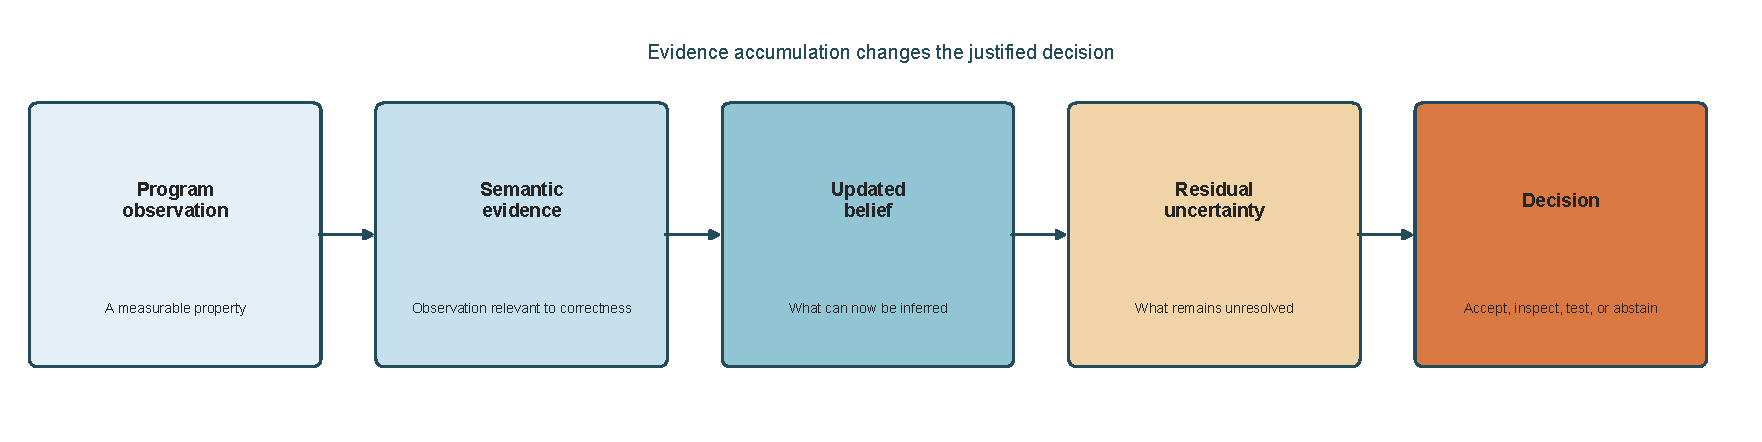
\includegraphics[width=.80\textwidth]{evidence_reasoning_chain.pdf}
\caption{Conceptual path from source--candidate observations to a verification decision. Observations update confidence, but residual uncertainty determines whether the system can act or must acquire stronger information.}
\label{fig:reasoning-chain}
\end{figure*}

Figure~\ref{fig:reasoning-chain} illustrates how these concepts relate during inference. Individual observations modify the confidence assigned to a candidate, while the remaining uncertainty determines whether that confidence is sufficient to support a decision. If the available evidence is inadequate, additional observations, or stronger forms of evidence, become necessary before action can be justified. Consequently, evidence accumulation is valuable only when it changes the decision that can reasonably be made.

The limits of the proposed representation can also be expressed formally. We define observational equivalence as
\begin{equation}
(s_i,c_i)\equiv_{\phi}(s_j,c_j)
\iff \phi(s_i,c_i)=\phi(s_j,c_j).
\label{eq:equivalence}
\end{equation}
Whenever two source--candidate pairs satisfy Equation~\ref{eq:equivalence} but correspond to different behavioral outcomes, every deterministic estimator operating only on $\phi$ must assign them the same prediction and therefore cannot classify both correctly. The resulting ambiguity is therefore an inherent consequence of the available observations rather than merely a limitation of the classifier. In other words, the irreducible uncertainty of EviCode arises from variation in the behavioral label $Y$ within the equivalence classes induced by $\phi$. Richer static analyses or formal reasoning may further refine these equivalence classes, whereas execution distinguishes them by revealing the behavior of the programs on concrete inputs.

\subsection{Semantic Obligations as Observable Compatibility}
A correct translation must satisfy several interacting obligations. It must be well formed, organize a complete computation, preserve decisions and repetition, perform compatible local operations, assign values compatible responsibilities, propagate information to compatible destinations, and invoke suitable target APIs. Table~\ref{tab:obligations} states what each family can expose and what remains hidden. EviCode maps these obligations to the vector in Equation~\ref{eq:evidence}.
\begin{equation}
\boldsymbol{e}(s,c)=\big[e_{\mathrm{lex}},e_{\mathrm{syn}},e_{\mathrm{str}},e_{\mathrm{ctl}},e_{\mathrm{op}},e_{\mathrm{role}},e_{\mathrm{flow}},e_{\mathrm{api}},e_{\mathrm{cx}}\big],
\label{eq:evidence}
\end{equation}
implemented by 45 scalar observations. Each family asks a memorable question. Did the same concepts appear? Can the candidate exist? Is computation organized compatibly? Can control proceed compatibly? Are local computations preserved? Do values retain responsibilities? Are values propagated compatibly? Are library choices plausible? Is the amount of computation compatible?
Each $e_{\mathrm{family}}$ in Equation~\ref{eq:evidence} is therefore a subvector rather than one scalar.

Language normalization does not assume that syntax or semantics are identical across languages. Each front end first maps language-specific constructs to shared computational concepts such as branches, loops, returns, calls, operator classes, and def--use roles. Scalar counts $a$ and $b$ are compared using the bounded agreement feature
\begin{equation}
r(a,b)=\frac{\min(a,b)}{\max(a,b,1)},
\label{eq:ratio}
\end{equation}
Equation~\ref{eq:ratio} gives maximal support to equal positive quantities, decreases support as the counts diverge, and assigns zero to joint absence rather than manufacturing agreement. Control, operator, statement, expression, and identifier-role profiles use cosine similarity. A shared absence can therefore remain part of a matched multivariate profile even though it does not independently add scalar evidence. These comparisons provide a common vocabulary, not invariance to every refactoring, library substitution, alias, or type-system difference.

\begin{table*}[t]
\centering
\caption{Semantic obligations represented by each observation family, the verification question each addresses, and its observational limit.}
\label{tab:obligations}
\begin{tabular}{@{}p{.12\textwidth}p{.22\textwidth}p{.27\textwidth}p{.29\textwidth}@{}}
\toprule
Family & Verification question & Failures it can expose & What remains hidden \\
\midrule
Lexical & Did related concepts appear? & Missing or unrelated content & Renaming and semantic substitutions \\
Syntax & Can the candidate exist structurally? & Truncation, malformed declarations & Compiling logical errors \\
Structure & Is computation organized compatibly? & Omitted blocks, unrelated organization & Correct refactoring and library replacement \\
Control flow & Can execution proceed compatibly? & Missing branches, loops, or returns & Wrong predicates in the same skeleton \\
Operators & Is local computation compatible? & Arithmetic, comparison, logical substitutions & Operand meaning and path conditions \\
Identifier roles & Do values retain responsibilities? & Changed identifier reuse and assignment, declaration, or call roles & Consistent renaming, aliases, and latent semantic roles \\
Data flow & Are values propagated compatibly? & Missing updates and suspicious dependencies & Heap state and path-sensitive flow \\
APIs & Are calls computationally plausible? & Hallucinated or mismatched methods & Equivalent APIs and wrong arguments \\
Complexity & Is a comparable amount of logic present? & Omitted reasoning or gratuitous machinery & Different computations of equal complexity \\
\bottomrule
\end{tabular}
\end{table*}

The final column is as important as the failure column. Every family can expose a class of disagreement, yet every family also leaves behaviorally decisive relations hidden. The taxonomy therefore organizes partial observations, not sufficient conditions for correctness.

\subsection{Operational Probe Design and Language Normalization}
The inventory was fixed before outcome analysis. Starting from the nine obligations in Table~\ref{tab:obligations}, a candidate extractor output was admitted only when it met five design rules. It had to be computable deterministically from both programs without labels, references, tests, or execution. It had to map to one declared verification question. It had to support a bounded or otherwise directly interpretable source--candidate comparison. It had to be available through the lightweight front ends used in this study. Finally, a component count and a profile-level comparison were both retained only when they answer different questions, such as whether the number of branches agrees and whether the overall control composition agrees. This process produced 53 exported quantities. It stopped at the declared lightweight boundary, excluding path-sensitive symbolic execution, alias and heap analysis, whole-program type proofs, and other analyses not supported consistently across the seven source languages.

We then apply an outcome-blind eligibility audit to all 53 outputs. An eligible output must obey the five rules and must not contain a correctness label, execution outcome, target reference, generator identity, or problem identifier. The pairwise relational boundary removes four unilateral quantities, namely absolute source and candidate length and separate source and candidate parser status. Their pairwise counterparts, length ratio and joint validity, remain. This choice studies compatibility between two programs instead of allowing task size, generator verbosity, or one-sided parser coverage to become direct predictors.

The remaining 49 pairwise outputs contain four formula-equivalent pairs. We retain one canonical channel from each pair: edit rather than retrieval similarity, normalized joint validity rather than its syntax proxy, normalized maximum AST-depth agreement rather than its raw duplicate, and normalized nesting agreement rather than its raw duplicate. The complete funnel is therefore 53 exported quantities, 49 pairwise quantities after the relational boundary, and 45 nonduplicate pairwise probes. The rules do not inspect correctness labels or held-out performance. Thus, 45 is the complete output of the declared construct and filtering process, not every program property that could be measured and not a claim that 45 is optimal, minimal, or statistically independent. Adding another probe would require a documented extension of the obligation map or extractor, followed by the same eligibility and redundancy audit.

Each program is analyzed independently by a language-parameterized front end. The implementation has parser-backed source profiles for Python and a Java parser for every candidate. The other six source languages use deterministic lexical and pattern-based control, operator, role, and approximate definition--use extractors. Parser-only comparisons contribute no positive support when the source parser is unavailable, and raw AST-node similarity falls back to lexical structure. RQ3 therefore includes a conservative sensitivity analysis that removes all six parser-dependent or parser-fallback channels. Where parsing is available, parser vocabulary is discarded in favor of validity, abstract-syntax-tree (AST) shape, declarations, and depth. Source and candidate quantities are compared only after mapping them to shared concepts. This normalization makes heterogeneous syntax comparable at the level of extracted properties. It does not make the languages semantically equivalent. Table~\ref{tab:inventory} inventories the probes. The artifact prefix \texttt{ln\_} marks normalized comparisons. Three surface controls and lower-level parser or token counters remain explicitly labeled so their contribution can be measured rather than conflated with deeper probes.

\begin{table*}[t]
\centering
\caption{Operational inventory of the 45 inference-time observations. Each row distinguishes the program property extracted in each language from the language-normalized comparison supplied to the estimator.}
\label{tab:inventory}
\begin{tabular}{@{}p{.105\textwidth}rp{.35\textwidth}p{.39\textwidth}@{}}
\toprule
Family & No. & Profile extracted & Source--candidate observations \\
\midrule
Surface controls & 3 & Tokens, text length, and edit sequence & Token Jaccard, edit similarity, and length ratio \\
Syntax & 1 & Joint parse/syntax success & Normalized joint validity \\
Structure & 12 & AST shape/depth where available, types, functions/classes, branching factor, statement/expression density and distributions & Raw structure controls plus normalized count, depth, density, and distribution agreement \\
Control flow & 11 & CFG count proxies, branches, loops, returns, exceptions, and control profile & Lower-level counters plus normalized component and profile agreement \\
Operators & 2 & Arithmetic, comparison, logical, and assignment families & Operator-pattern and normalized operator-family similarity \\
Identifier roles & 6 & Identifier identity, count/entropy, and approximate assignment, declaration, and call roles & Raw identity and role agreement plus normalized count and role-distribution agreement \\
Data flow & 4 & Approximate definitions, uses, reads/writes, and assignments & Broad relation, def--use count, read/write ratio, and assignment-density similarities \\
APIs and calls & 4 & Extracted method/library names, mismatches, and call count & API and call-name overlap, API mismatch, and normalized call-count agreement \\
Complexity & 2 & Cyclomatic complexity and maximum nesting & Normalized complexity and nesting agreement \\
\midrule
\textbf{Total} & \textbf{45} & \multicolumn{2}{l}{No label, execution result, compiler outcome, generator, problem ID, or target reference is included.} \\
\bottomrule
\end{tabular}
\end{table*}

The training partition provides a final quality-control audit without changing the construct rules. All 45 observations have complete numerical coverage and nonzero variance. No pair is exactly duplicated, and the standardized matrix has rank 45, meaning that no probe can be reconstructed exactly as a linear combination of the others. This rules out exact linear redundancy, not statistical dependence or semantic overlap. Spearman correlation measures whether two probes tend to rise and fall together without assuming a linear relation. Twelve pairs have absolute correlation of at least 0.90. Ten connect alternate control or tree-profile measurements, while the remaining pairs connect call overlap with API mismatch ($0.940$) and token overlap with identifier overlap ($0.919$). Linking these pairs forms 36 dependence groups, the largest containing four probes. We retain correlated probes when they use different extraction paths or answer different obligations because they can fail differently when parsing or normalization is incomplete. RQ3 therefore tests a 36-probe correlation-pruned basis, a parser-independent basis, and an expanded duplicate-inclusive basis instead of assuming independence. We do not separately validate extraction accuracy for every construct in every language. A named coordinate is traceable to the extracted property, but that traceability is not proof that a lightweight front end recovered the intended semantic construct perfectly.

For intuition, Table~\ref{tab:normalized-example} traces a Python clamp function and its Java candidate through the extractor. Each front end first records language-specific constructs and then maps them to shared properties. The source--candidate comparison becomes a value between 0 and 1 in the 45-dimensional vector. A value of 1 denotes maximal agreement for that observation, whereas 0 denotes no positive support. Neither value is a correctness probability. The Java class wrapper required for parsing is omitted from the snippets but retained when computing every value.

\begin{table*}[t]
\centering
\caption{Worked example showing how language-specific constructs become bounded source--candidate observations. Each value measures agreement in one extracted property. It is neither a correctness probability nor proof of equivalence.}
\label{tab:normalized-example}
\small
\setlength{\tabcolsep}{5pt}
\begin{tabular}{@{}>{\raggedright\arraybackslash}p{.21\textwidth}>{\raggedright\arraybackslash}p{.24\textwidth}>{\raggedright\arraybackslash}p{.23\textwidth}>{\raggedright\arraybackslash}p{.24\textwidth}@{}}
\toprule
What Python contains & What Java contains & What EviCode records & Value and plain meaning \\
\midrule
\texttt{def clamp(value, lower, upper):} & \texttt{static int clamp(int value, int lower, int upper)\{} & Both programs parse and contain one routine & Joint validity $=1.000$ \newline Function-count agreement $=1.000$ \\
Two \texttt{if} conditions and one \texttt{return} & Two \texttt{if} conditions and one \texttt{return} & Control profile and decision-based complexity & Control-profile agreement $=1.000$ \newline Complexity agreement $=1.000$ \\
\texttt{result = value}, \texttt{<}, and \texttt{>} & \texttt{result = value}, \texttt{<}, and \texttt{>} & Three assignments and two comparison directions in each & Operator-pattern agreement $=1.000$ \newline Operator-family agreement $=1.000$ \\
\texttt{clamp}, \texttt{value}, \texttt{lower}, \texttt{upper}, \texttt{result} & The same task names plus Java type and wrapper names & Identifier identity and assignment, declaration, and call-role profiles & Identifier overlap $=0.714$ \newline Role-distribution agreement $=0.943$ \\
\texttt{result} receives \texttt{value}, \texttt{lower}, and \texttt{upper} & \texttt{result} receives the same three values & Three approximate definition--use relations & Data-flow overlap $=1.000$ \newline Def--use count agreement $=1.000$ \\
Untyped parameters and result & Parameters and result declared as \texttt{int} & Declared type and signature-token overlap & Type agreement $=0.000$ \newline No comparable source type was observed \\
\bottomrule
\end{tabular}
\end{table*}

The example shows why counts alone are insufficient and why low agreement is not automatically a defect. If the Java candidate changes the first \texttt{<} to \texttt{>} and changes \texttt{result = lower} to \texttt{result = upper}, its control-profile and complexity agreements remain 1.000. Operator-pattern agreement falls to 0.707 and data-flow overlap falls to 0.667 because different local computations and dependencies are now observed. Conversely, Java wrapper and type syntax lower identifier and type agreement in the plausible pair. The observations therefore expose different kinds of agreement and disagreement, but only behavioral evidence can establish what the program does on concrete inputs.

\subsection{Conceptual Semantic Observability Stratification}
Equation~\ref{eq:hierarchy} organizes the probes by the kind of program object they inspect
\begin{equation}
\begin{aligned}
\mathcal{O}=\big[&\{\text{surface}\},\{\text{validity}\},\{\text{structure}\},\\
&\{\text{control},\text{operators},\text{roles}\},\\
&\{\text{flow},\text{APIs}\},\{\text{behavior}\}\big] .
\end{aligned}
\label{eq:hierarchy}
\end{equation}
A later group observes a more relational object closer to behavior. Surface records representation, validity establishes analyzability, and structure records organization. Control, operators, and roles are parallel views of execution shape, local computation, and value responsibility. Flow and APIs add relations among values or invoked abstractions, while behavior observes concrete outcomes. Roles precede flow because they describe local responsibilities, whereas flow relates definitions and uses, not because experiments assign roles lower AUC. Complexity is cross-cutting because it summarizes organization without introducing a distinct semantic object.

Equation~\ref{eq:hierarchy} is a conceptual stratification, not an empirically inferred total order. Families within braces are unordered, adjacent groups overlap, and strict information inclusion is not claimed. Its basis is semantic granularity and proximity to runtime relations, independent of fitted importance or AUC. Lower-level probes can be more predictive when generators leave recurring surface traces. The experiments test association, replacement, transport, and ambiguity under this organization. They do not establish that acquiring every successive group must monotonically improve a model.

Behavior is included to mark the observability boundary, but it is not among the 45 inference observations. The experiments use execution only for supervision and ground truth. RQ2 conditions on compilation and measures how the same instrument behaves when validity no longer separates the classes. RQ3 measures overlap and complementarity among static families, then compares their explicit representation with frozen pretrained encoders. Grade progression tests whether higher behavioral quality produces monotonic static agreement. Figure~\ref{fig:continuum} later synthesizes the resulting Semantic Information Ladder as an acquisition perspective rather than a measured performance sequence.

\subsection{Transparent Learning Instrument}
The primary instrument, denoted EviCode-LR, estimates
\begin{equation}
\hat p_\theta(s,c)=\sigma\!\left(\beta_0+\sum_{j=1}^{45}\beta_j z_j(s,c)\right),
\label{eq:model}
\end{equation}
In Equation~\ref{eq:model}, $\beta_0$ is the intercept, $\beta_j$ is the fitted contribution weight, $z_j$ is a standardized observation, and $\sigma$ converts log-odds to probability. Logistic regression is selected for auditability, not as a modeling innovation. Its additive form exposes the conditional use of each observation. The principal, transfer, calibration, and worked-profile results all use EviCode-LR. EviCode-XGB appears only in the capacity sensitivity analysis and does not replace the transparent instrument. Mutual information asks what a probe predicts alone, while linear SHAP attribution asks how far a probe moves fitted log-odds relative to its training mean. Family ablation measures what the system loses when related probes disappear.

For deployment domain $d$, calibration requires more than a useful score ordering:
\begin{equation}
P_d(Y=1\mid \hat p=p)=p.
\label{eq:domaincal}
\end{equation}
The domain subscript in Equation~\ref{eq:domaincal} makes the dependency explicit. A representation can preserve relative evidence under language or generator shift while $P_d(Y\mid Z)$ changes, invalidating a threshold or probability learned in another domain. This distinction motivates separate transfer and reliability RQs.

\section{Research Questions}
Five RQs form one investigation rather than five independent benchmarks.

\textbf{RQ1: Signal existence.} \emph{Do execution-labelled translation outcomes reveal a recoverable static signal about functional correctness?} This establishes whether a source--candidate pair contains useful non-behavioral information.

\textbf{RQ2: Conditional observability.} \emph{What remains observable after non-compiling failures are removed?} Applying the same estimator to compiling incorrect and correct candidates tests a behavior-proximal population.

\textbf{RQ3: Representation and attribution.} \emph{How is correctness-related support distributed, and what is gained or lost relative to pretrained code representations?} Basis checks, attribution, ablation, learner capacity, embedding comparisons, progression, and cases test predictive strength and traceability together.

\textbf{RQ4: Domain transport.} \emph{Do learned source--candidate relationships transport across source languages and generators?} Problem-disjoint transfer and domain-exclusion retraining test complementary forms of distribution shift.

\textbf{RQ5: Probability meaning.} \emph{When can a static score be read as a reliable probability of correctness?} Calibration tests whether useful ranking also supports deployment decisions.

RQ1 first establishes a signal. RQ2 removes easy static failures. RQ3 identifies and benchmarks the representation behind that signal. RQ4 tests whether it survives domain change, and RQ5 determines whether its magnitude remains decision-relevant.

With the inference boundary and questions fixed, the next requirement is a dataset where generated successes and failures are established behaviorally without placing behavior in the model input.

\section{Experimental Design}
\subsection{Execution-Grounded Translation Outcomes}
The analysis dataset contains 30,979 translations from C, C++, C\#, Python, Ruby, Kotlin, and Swift to Java, generated by DeepSeek-Coder, QwenCoder, and StarCoder. Every row is a complete generator output, and no mutation is added to create failures. We import the released CodeNetTrans-QS execution grades and do not reconstruct the benchmark oracle.

Fixing Java is a deliberate control. It holds candidate parsing, target APIs, wrapper conventions, the compiler and runtime, and the behavioral setting constant while source syntax and generator vary. RQ4 can therefore examine source and generator transport without a simultaneous target-language change. Source inclusion depends on extractor and dataset coverage, not EviCode performance. Each retained language has a front end, occurs under all three generators, and contributes 1,184--6,228 eligible Score-1-to-3 records. The only other source label, Haxe, has 103 eligible records, only three Score-3 StarCoder outputs, and no front end. Including it would confound language effects with severe sparsity and extractor availability. The design controls source-language variation but cannot establish target-language independence.

Table~\ref{tab:data} reports the exact marginals because language, generator, and grade imbalance affect thresholds and calibration. Score 1 denotes parsable but non-compilable output, Score 2 denotes compilable output that fails the behavioral oracle, and Score 3 denotes observed functional success under that oracle. Scores 1 and 2 form the negative class, while Score 3 forms the positive class. This definition makes the primary task estimation of execution-grounded correctness under the benchmark oracle. Score 2 versus 3 is a conditional, behavior-proximal evaluation.

\begin{table*}[t]
\centering
\caption{CodeNetTrans-QS composition by source language, generator, and execution grade. Score 1 is parsable but non-compiling, Score 2 compiles but fails behavioral evaluation, and Score 3 passes the dataset oracle.}
\label{tab:data}
\begin{tabular}{@{}lrrrr@{\qquad}lrrrr@{}}
\toprule
Source language & Score 1 & Score 2 & Score 3 & Total & Generator & Score 1 & Score 2 & Score 3 & Total \\
\midrule
C      & 3,016 & 1,090 & 1,366 & 5,472 & DeepSeek-Coder & 2,980 & 3,770 & 4,654 & 11,404 \\
C++    & 2,501 & 1,081 & 1,554 & 5,136 & QwenCoder      & 5,464 & 1,779 & 1,692 & 8,935 \\
C\#   & 3,306 &   588 &   767 & 4,661 & StarCoder      & 8,260 & 1,555 &   825 & 10,640 \\
Python & 3,104 & 1,727 & 1,397 & 6,228 & \textbf{All} & \textbf{16,704} & \textbf{7,104} & \textbf{7,171} & \textbf{30,979} \\
Ruby   & 2,509 & 1,743 &   915 & 5,167 & & & & & \\
Kotlin & 1,861 &   561 &   709 & 3,131 & & & & & \\
Swift  &   407 &   314 &   463 & 1,184 & & & & & \\
\bottomrule
\end{tabular}
\end{table*}

Three imbalances shape every later result. Non-compiling failures constitute 53.9\% of the analysis set, so the primary task rewards validity evidence. Correctness prevalence is 40.8\% for DeepSeek-Coder, 18.9\% for QwenCoder, and 7.8\% for StarCoder, making one pooled threshold potentially misleading. Python supplies 20.1\% of the data, while Swift supplies 3.8\%, so pooled metrics emphasize larger languages. Problem-disjoint evaluation prevents task overlap, but it does not remove these distributional differences.

Problems, rather than rows, are assigned once to a 70/30 partition with seed 42. The training partition contains 21,497 rows from 2,664 problems, and the test partition contains 9,482 rows from 1,142 different problems. This prevents task overlap from explaining the primary result. EviCode-LR is standardized on the training partition and fitted without class weighting or post-hoc calibration. The Score-2-versus-3 evaluation filters the test rows after fitting, so it measures how the primary model behaves under a changed population rather than a separately trained hard-task model. Confidence intervals use 500 bootstrap samples of test problems. They quantify test-sample uncertainty conditional on this split and fitted model, not variability across training seeds. ROC-AUC and average precision (AP) test ordering. Precision, recall, and F1 test the fixed 0.5 acceptance boundary. Brier score and ten-bin expected calibration error (ECE) test probabilistic meaning. Domain metadata defines partitions but never enters the feature matrix.

\subsection{Evaluation Logic}
Each metric answers a different scientific question. Let $\hat p^+$ and $\hat p^-$ denote EviCode scores for randomly selected correct and incorrect translations. ROC-AUC measures threshold-independent ordering:
\begin{equation}
\mathrm{ROC\mbox{-}AUC}=P(\hat p^+>\hat p^-)+\frac{1}{2}P(\hat p^+=\hat p^-).
\label{eq:rocauc}
\end{equation}
Equation~\ref{eq:rocauc} makes ROC-AUC the probability that EviCode ranks the correct member of a correct--incorrect pair higher, with ties receiving half credit. A value of $0.5$ denotes random ordering and $1.0$ perfect ordering. Average precision summarizes how concentrated correct candidates remain near the top of the ranking:
\begin{equation}
\mathrm{AP}=\sum_{k=1}^{K}(R_k-R_{k-1})P_k,
\label{eq:ap}
\end{equation}
In Equation~\ref{eq:ap}, $P_k$ and $R_k$ are precision and recall at the $k$th ranked threshold. AP is the discrete summary computed by the evaluation library rather than a trapezoidal precision--recall integral. Its no-skill baseline equals correctness prevalence, so AP is compared only across samples with compatible class balance.

Ranking alone does not specify which candidates EviCode would accept. At threshold $\tau=0.5$, the decision for candidate $i$ is $\hat y_i(\tau)=\mathbb{1}[\hat p_i\geq\tau]$. Let TP and FP count accepted candidates that are correct and incorrect, respectively, and let FN count correct candidates that are rejected. The threshold metrics are
\begin{equation}
\begin{gathered}
\mathrm{Precision}=\frac{\mathrm{TP}}{\mathrm{TP}+\mathrm{FP}},\qquad
\mathrm{Recall}=\frac{\mathrm{TP}}{\mathrm{TP}+\mathrm{FN}},\\
\mathrm{F1}=2\frac{\mathrm{Precision}\cdot\mathrm{Recall}}
{\mathrm{Precision}+\mathrm{Recall}}.
\end{gathered}
\label{eq:thresholdmetrics}
\end{equation}
Equation~\ref{eq:thresholdmetrics} separates three threshold-dependent questions. Precision asks how trustworthy an EviCode acceptance is, recall asks how many correct candidates the threshold retains, and F1 balances these objectives. All three depend on $\tau$ and describe one operating point rather than the full ranking.

Probability metrics ask whether the numerical score itself is meaningful. For $n$ candidates with correctness labels $y_i\in\{0,1\}$ and predicted probabilities $\hat p_i$, the Brier score
\begin{equation}
\mathrm{BS}=\frac{1}{n}\sum_{i=1}^{n}(\hat p_i-y_i)^2
\label{eq:brier}
\end{equation}
is the mean squared error of the predicted correctness probabilities. It ranges from $0$ for perfect probability forecasts to $1$ for maximally wrong forecasts. Lower values mean that EviCode's confidence is closer to the observed outcomes. Expected calibration error
\begin{equation}
\mathrm{ECE}=\sum_{b=1}^{B}\frac{|I_b|}{n}\left|\mathrm{acc}(I_b)-\mathrm{conf}(I_b)\right|
\label{eq:ece}
\end{equation}
summarizes the gap between confidence and observed correctness over $B=10$ equal-width bins. Here, $I_b$ is the set of predictions in bin $b$, $\mathrm{acc}(I_b)=|I_b|^{-1}\sum_{i\in I_b}y_i$ is their observed correctness rate, and $\mathrm{conf}(I_b)=|I_b|^{-1}\sum_{i\in I_b}\hat p_i$ is their mean EviCode confidence. An ECE of $0$ is ideal. For example, predictions assigned confidence $0.70$ are calibrated when approximately $70\%$ are correct. Equations~\ref{eq:brier} and \ref{eq:ece} evaluate probability quality rather than ranking. For EviCode, a strong AUC with weak calibration would still support candidate prioritization, but it would not justify interpreting a score as a correctness probability. ECE is therefore interpreted with reliability diagrams because a small pooled average can conceal domain-specific or sparsely populated errors.

Table~\ref{tab:metric-reading} provides hypothetical values so later results can be interpreted without treating AUC, F1, or calibration error as interchangeable.

\begin{table}[t]
\centering
\caption{How to interpret EviCode evaluation metrics. Values are hypothetical illustrations, not experimental results.}
\label{tab:metric-reading}
\footnotesize
\begin{tabular}{@{}p{0.15\columnwidth}p{0.20\columnwidth}p{0.51\columnwidth}@{}}
\toprule
Metric & Example & Meaning for EviCode \\
\midrule
ROC-AUC & $0.80$ & Correct ranks higher in $80\%$ of random correct--incorrect pairs; not $80\%$ accuracy. \\
AP & $0.50$ (prevalence $0.25$) & Correct candidates concentrate above the prevalence baseline; not a correctness rate. \\
Precision & $0.70$ & $70\%$ of accepted candidates are correct. \\
Recall & $0.60$ & $60\%$ of all correct candidates are accepted. \\
F1 & $0.65$ & Harmonic balance of precision and recall; not accuracy. \\
Brier & $0.15$ & Mean squared probability error; $0$ is ideal. \\
ECE & $0.05$ & The bin-weighted absolute confidence gap averages $5$ percentage points; $0$ is ideal. \\
\bottomrule
\end{tabular}
\end{table}

\subsection{Diagnostic Visualization Protocol}
The additional visual analyses preserve the primary problem-disjoint partition. In each transfer-matrix cell, EviCode-LR is fitted only to training-partition rows from the row domain and evaluated only on test-partition rows from the column domain. No problem crosses the global partition. Diagonal cells are within-domain held-out evaluations, whereas off-diagonals measure single-domain transfer to unseen problems. These matrices are diagnostic and are not accompanied by multiple pairwise significance claims.

Leave-one-language-out and leave-one-generator-out (LOGO) models provide external generalization checks under domain exclusion. The leave-one-generator-out evaluation tests whether semantic relationships learned from two LLM families transfer to a previously unseen code generator. The leave-one-language-out evaluation tests whether the representation remains useful when an entire source language is excluded during training. A held-out task may still appear through another language or generator, so LOGO complements rather than replaces the problem-disjoint transfer matrices.

Generator reliability curves use eight quantile bins so each point has comparable support. The accompanying densities are normalized within correctness class. Family correlations are Pearson correlations between per-pair family means on the held-out partition. Violin plots sample up to 1,500 pairs per grade with a fixed seed, preventing the majority grade from dominating the display.

\subsection{Feature-Basis Validation}
Selection and dependence checks use only the training partition. Exact equality identifies operational duplicates. For sensitivity analysis, absolute Spearman correlation at a conservative 0.90 threshold flags probes with nearly identical monotonic movement. A deterministic pass considers normalized channels first and removes any later channel correlated at or above 0.90 with one already retained, leaving 36 probes. A separate 39-probe variant removes every parser-dependent or parser-fallback channel. We then fit the same standardized Logistic Regression to these reduced bases, the declared 45-probe basis, all 49 pairwise outputs including duplicates, and broader variants that restore unilateral quantities. The 0.90 threshold never determines the declared basis. Held-out results diagnose sensitivity and are not used to select 45. Paired 95\% confidence intervals resample complete programming problems 500 times.

\subsection{Same-Information Baselines}
Reference-free alternatives must receive the same source program and generated candidate without execution, tests, a target reference, problem text, or generator metadata. We therefore compare EviCode with controlled models trained on the identical problem-disjoint split. The class-prior baseline supplies no ranking information. Token overlap uses only Jaccard similarity. Surface evidence adds edit similarity and length ratio. Validity uses only source--candidate parser validity. The unnormalized-static baseline uses the 17 conventional cross-language similarity proxies, while the language-normalized baseline uses only the 28 shared computational observations. A final stress test removes all surface and validity features. Every learned baseline uses the same standardized logistic regression, seed, labels, and 0.5 threshold as EviCode. ROC-AUC intervals use the same 500 problem-clustered bootstrap samples.

RQ3 crosses five representations with seven learners on the same split and labels. EviCode supplies 45 explicit observations. The frozen checkpoints are \texttt{microsoft/codebert-base}, \texttt{microsoft/graphcodebert-base}, \texttt{microsoft/unixcoder-base}, and \texttt{Salesforce/codet5-small}~\cite{feng2020codebert,guo2021graphcodebert,guo2022unixcoder,wang2021codet5}. Their pretrained weights are not updated. Each independently encodes the source and candidate up to 256 tokens. Mean-pooled vectors are combined by absolute difference, elementwise product, and cosine similarity. GraphCodeBERT is used without its specialized data-flow graph. Logistic Regression, Random Forest, Extra Trees, histogram gradient boosting, XGBoost, LightGBM, and a two-layer multilayer perceptron use one fixed representative configuration each across all representations, with no representation-specific search. The full matrix is exploratory, and its paired intervals are not adjusted for selecting the strongest of 35 combinations. It is a controlled frozen-representation comparison rather than reproduction of every specialized architecture.

This design first asks whether execution-grounded supervision produces a reusable static signal. It then conditions on a harder population, tests how the signal is distributed and represented, examines domain transport, and finally checks whether score magnitude retains probability meaning.

\section{RQ1: Does Recoverable Evidence Exist?}
\label{sec:rq1}
The first question is intentionally fundamental. Does a source--candidate pair contain any useful static signal about behavioral correctness? If not, no learner using this inference boundary could prioritize candidates. RQ1 tests that premise on programming problems completely absent from training.

Table~\ref{tab:main} shows that EviCode-LR distinguishes correct from incorrect translations on unseen problems without observing execution or compiler outcomes. ROC-AUC is 0.790 (95\% confidence interval (CI) [0.777, 0.804]), so a random correct candidate outranks a random incorrect one approximately 79.0\% of the time. This result establishes an aggregate, reusable signal. RQ3 determines which probes the fitted model uses. F1 is 0.392 because ranking and accepting are different tasks. The fixed 0.5 boundary retains only 28.2\% of correct candidates even though their relative ordering is useful. The Brier score of 0.141 also improves on the approximately 0.176 error of a constant forecast equal to test prevalence. Pooled ECE of 0.011 describes the matched mixture and does not imply equal reliability within every domain.

\begin{table}[t]
\centering
\caption{EviCode-LR on 9,482 translations from unseen problems. The primary task compares Score 3 with Scores 1--2. The conditional task applies the same fitted model only to compiling Scores 2--3 and is interpreted in RQ2.}
\label{tab:main}
\begin{tabular}{@{}lcc@{}}
\toprule
Metric & Primary task & Score 2 vs. 3 \\
\midrule
ROC-AUC & 0.790 & 0.687 \\
AP & 0.537 & 0.692 \\
Precision & 0.645 & 0.778 \\
Recall & 0.282 & 0.282 \\
F1 & 0.392 & 0.414 \\
Brier & 0.141 & 0.254 \\
ECE & 0.011 & 0.177 \\
\bottomrule
\end{tabular}
\end{table}

\begin{table}[t]
\centering
\caption{Same-information baseline comparison by ROC-AUC. Every method receives only the source and candidate. The conditional task compares compiling incorrect Score-2 outputs with correct Score-3 outputs.}
\label{tab:baselines}
\begin{tabular}{@{}lcc@{}}
\toprule
Observation set & Primary task & Conditional task \\
\midrule
Class prior & 0.500 & 0.500 \\
Token overlap only & 0.656 & 0.489 \\
Surface only & 0.666 & 0.518 \\
Validity only & 0.536 & 0.497 \\
Unnormalized static & 0.756 & 0.645 \\
Language-normalized only & 0.764 & 0.674 \\
No surface or validity & 0.784 & 0.684 \\
EviCode full & \textbf{0.790} & \textbf{0.687} \\
\bottomrule
\end{tabular}
\end{table}

Table~\ref{tab:baselines} rules out two simple explanations for the primary result. Token overlap alone reaches 0.656 AUC and joint validity alone reaches 0.536, well below the full model's 0.790. Language-normalized probes alone retain 0.764, while removing every surface and validity probe still yields 0.784. The 0.006 difference between this reduced basis and the full representation shows that most primary-task ordering is not supplied by token matching or joint parser validity. These same-information baselines establish incremental value over transparent alternatives. RQ2 examines the conditional column, and RQ3 separately compares frozen encoders under a standardized protocol.

The results should be interpreted from two complementary perspectives. ROC-AUC evaluates how well the estimator orders candidates, whereas F1 evaluates how effectively one fixed threshold balances accepted correct candidates against missed correct candidates. Strong ordering can therefore coexist with modest recall. Such a model can prioritize review or testing, but the 0.5 threshold is not automatically a suitable deployment policy.

\textbf{Answer to RQ1.} Source--candidate observations contain a recoverable signal about execution-grounded correctness. EviCode-LR ranks a correct translation above an incorrect one in approximately 79\% of random correct--incorrect pairs, with a problem-clustered interval of [0.777, 0.804]. This supports prioritization on unseen problems, not proof or autonomous acceptance. Having established a signal, RQ2 asks what the same model retains when non-compiling failures are removed.

\section{RQ2: What Remains Observable After Compilation?}
\label{sec:rq2}
The conditional evaluation in Table~\ref{tab:main} retains the EviCode-LR model trained on Scores 1--3 and applies it only to test candidates that compile. It therefore asks whether the original static score remains informative after changing the evaluated population. ROC-AUC decreases from 0.790 to 0.687 (95\% CI [0.669, 0.704]). This is a population contrast, not an ablation and not a causal estimate of how much information compilation contributes. It shows that the current 45-probe linear instrument has less discrimination once non-compiling cases no longer separate the classes.

The transparent baselines help clarify the origin of the remaining predictive signal. Token overlap and joint validity achieve ROC-AUC values of only 0.489 and 0.497, respectively, which are close to random performance. Introducing the language-normalized semantic probes increases the ROC-AUC to 0.674, while the complete representation reaches 0.687. These comparisons indicate that the residual ranking capability cannot be attributed simply to identifying compilable programs. Instead, it arises from semantic information captured by the proposed representation.

Probability estimation degrades more noticeably under the same conditions. The compiling subset contains 2,164 correct translations among 4,374 candidates and is therefore nearly balanced. Consequently, its average precision (0.692) is not directly comparable with the primary-task average precision of 0.537, where the class distribution differs substantially. Calibration quality also deteriorates. The Brier score increases to 0.254, slightly worse than the approximate error of 0.250 obtained by predicting the class prevalence for every instance, while the expected calibration error (ECE) rises to 0.177 because the model trained on the full dataset is applied to the conditioned population without recalibration. Although the F1 score shows a small increase, this improvement results from the altered class prevalence and the unchanged operating threshold rather than from a genuine increase in discriminative ability. In other words, the conditioned task itself does not become easier to solve.

Compilation verifies only that a program satisfies the requirements of the language toolchain. It provides no assurance that loops iterate over the correct range, boundary conditions are handled appropriately, accumulated values are propagated correctly, or the implemented algorithm preserves the intended behaviour of the source program. The present results should therefore not be interpreted as a fundamental limit of static reasoning. Rather, they quantify the capabilities of the lightweight semantic representation used in EviCode under the evaluated learners and benchmark. More sophisticated static analyses, symbolic reasoning techniques, or formal verification methods may further reduce the remaining ambiguity.

\textbf{Answer to RQ2.} EviCode-LR continues to provide useful ranking information even when evaluation is restricted to compiling candidates, achieving a ROC-AUC of 0.687 (95\% CI [0.669, 0.704]). In contrast, the associated probability estimates no longer remain well calibrated for the conditioned population. These findings suggest that static semantic evidence is still valuable for prioritizing candidates for testing or manual review, but it should not be interpreted as evidence of correctness. Distinguishing cases that remain ambiguous under the current representation requires additional behavioural or formal evidence. This observation naturally motivates RQ3, which investigates how the available static information is distributed across the representation and whether stronger learning algorithms or pretrained representations can exploit that information more effectively.

\section{RQ3: What Does an Explicit Representation Provide?}
\label{sec:rq3}
RQ3 investigates how the available static semantic information is distributed across the representation and how effectively different learning methods exploit it. The analysis is organized into five complementary stages. We first examine \emph{basis sensitivity} to determine whether the reported performance depends critically on selecting exactly 45 probe dimensions. Next, \emph{feature attribution} and \emph{probe-family ablation} distinguish the information actively used by the model from information that can be replaced by other observations. We then evaluate a \emph{representation--learner matrix} to assess whether the conclusions are specific to Logistic Regression or whether stronger learners and frozen pretrained code encoders extract substantially different information from the same representation. The fourth analysis studies \emph{grade progression}, asking whether increasing correctness simply reflects increasing similarity between the source and candidate programs. Finally, we combine \emph{statistical dependence analysis} with detailed worked examples to identify both the explanatory power and the limitations of the named semantic probes.

\subsection{Basis Size and Dependence}
Before interpreting the contribution of individual probes, we first examine whether the reported results depend on using exactly 45 observation dimensions. Table~\ref{tab:feature-basis} summarizes this analysis. The first four configurations preserve the same pairwise compatibility prediction task while modifying the basis used to represent each source--candidate pair.

\begin{table}[!t]
\centering
\caption{Feature-basis sensitivity on the same problem-disjoint split. Primary AUC compares Score 3 with Scores 1--2, while conditional AUC evaluates compiling Scores 2--3. The first four variants preserve pairwise compatibility. Each 47-probe row independently adds two unilateral quantities, while all 53 outputs combine unilateral and duplicate channels.}
\label{tab:feature-basis}
\footnotesize
\setlength{\tabcolsep}{3.4pt}
\begin{tabular}{@{}lrrr@{}}
\toprule
Observation basis & Probes & Primary AUC & Conditional AUC \\
\midrule
Correlation-pruned pairwise & 36 & 0.787 & 0.685 \\
Without parser channels & 39 & 0.788 & 0.688 \\
\textbf{Declared pairwise inventory} & \textbf{45} & \textbf{0.790} & \textbf{0.687} \\
Pairwise including duplicates & 49 & 0.790 & 0.687 \\
Plus unilateral validity & 47 & 0.811 & 0.697 \\
Plus absolute lengths & 47 & 0.830 & 0.730 \\
All extractor outputs & 53 & 0.840 & 0.736 \\
\bottomrule
\end{tabular}
\end{table}

Removing nine highly correlated probes through correlation pruning changes the primary-task ROC-AUC by only $-0.0025$ (95\% CI [${-0.0048}$, ${-0.0003}$]). Although these correlated probes contribute a small amount of additional information, a reduced representation containing 36 probes retains almost the entire ranking capability of the original model.

We next remove all six parser-dependent or parser-fallback probes, leaving a representation of 39 probes. Under this configuration, the primary-task ROC-AUC remains 0.788, while the conditional-task ROC-AUC is 0.688. These results demonstrate that the overall ranking performance is largely preserved even without parser-dependent information. However, this finding should not be interpreted as evidence that extraction quality is identical across programming languages, nor does it exclude language-specific effects within the remaining probe set.

Finally, restoring four intentionally duplicated probe channels changes the ROC-AUC by only $+0.0001$ (95\% CI [${-0.00002}$, 0.00027]). The negligible difference confirms that duplicate measurements do not account for the observed predictive performance.

The broader variants expose an important construct trade-off. Adding separate source and candidate parser outcomes raises AUC from 0.790 to 0.811, an absolute increase of 0.022 [0.017, 0.026]. Adding absolute source and candidate lengths raises AUC to 0.830, an absolute increase of 0.040 [0.033, 0.047]. Restoring every output reaches 0.840, an absolute increase of 0.050 [0.042, 0.058]. These gains answer whether a candidate is likely to be correct given its size and one-sided validity, not only whether source and candidate agree. Length can encode task size or generator verbosity, source parser status can expose language coverage, and target parser status can act as a direct validity cue. We therefore retain the 45-probe basis for construct alignment rather than maximum benchmark AUC. It is the complete de-duplicated pairwise inventory under the stated boundary, not an independent, minimal, or universally optimal semantic basis.

\subsection{Distributed Explanatory Support}
RQ3 next asks whether the RQ1 signal comes from one dominant probe or several partially replaceable constraints. For a linear model with standardized inputs, a SHAP value is the probe's signed movement of log-odds relative to its training mean. Mean absolute SHAP therefore measures typical contribution magnitude without treating direction as importance. Figure~\ref{fig:families} reports the ten largest training-partition values. Table~\ref{tab:importance-views} compares this conditional view with standardized coefficient magnitude and marginal mutual information.

\begin{table}[t]
\centering
\caption{Leave-one-family-out ablation on the fixed problem-disjoint split. Deltas are point estimates relative to EviCode-LR, and negative values denote loss. No family removal reduces AUC by more than 0.009, indicating distributed, partially replaceable support.}
\label{tab:ablation}
\begin{tabular}{@{}lrrr@{}}
\toprule
Removed family & AUC & $\Delta$AUC & $\Delta$F1 \\
\midrule
Control flow & 0.781 & $-0.009$ & $-0.041$ \\
APIs         & 0.783 & $-0.007$ & $-0.042$ \\
Structure    & 0.785 & $-0.005$ & $-0.029$ \\
Complexity   & 0.785 & $-0.005$ & $-0.015$ \\
Surface      & 0.786 & $-0.004$ & $-0.013$ \\
Data flow    & 0.787 & $-0.003$ & $-0.011$ \\
Identifiers  & 0.787 & $-0.003$ & $-0.016$ \\
Syntax       & 0.788 & $-0.002$ & $-0.008$ \\
Operators    & 0.790 & $<-0.001$ & $-0.004$ \\
\bottomrule
\end{tabular}
\end{table}

\begin{figure}[t]
\centering
\makebox[\linewidth][c]{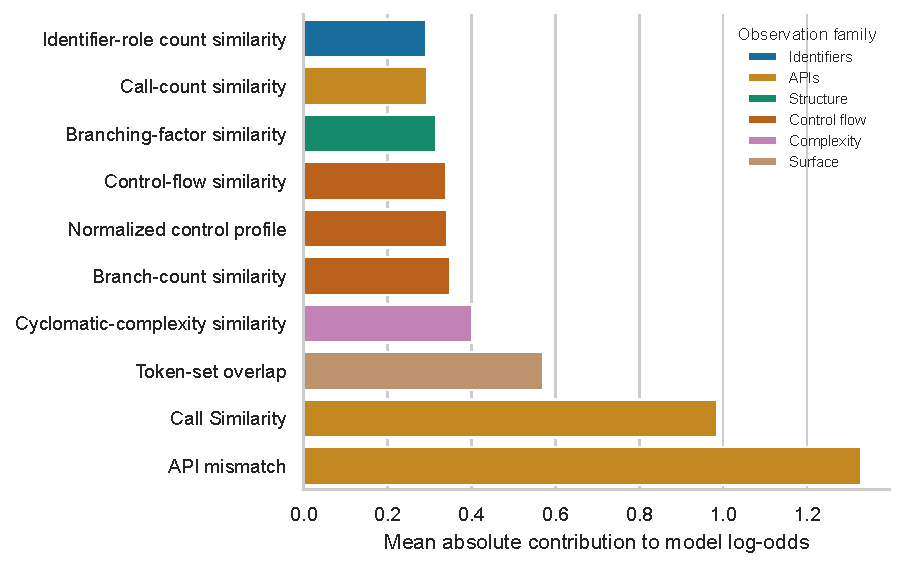
\includegraphics[width=1.04\linewidth]{evidence_importance.pdf}}
\caption{Ten probes with the largest mean absolute linear SHAP values on the training partition. Longer bars indicate greater typical movement of EviCode-LR log-odds, not greater semantic depth, causal importance, or irreplaceability.}
\label{fig:families}
\end{figure}

\begin{table}[t]
\centering
\caption{Three complementary importance views. SHAP and coefficient magnitude describe conditional model use, while mutual information (MI) measures one-probe marginal association.}
\label{tab:importance-views}
\footnotesize
\setlength{\tabcolsep}{3pt}
\begin{tabular}{@{}p{.18\columnwidth}p{.53\columnwidth}p{.17\columnwidth}@{}}
\toprule
View & Three highest-ranked probes & Values \\
\midrule
Linear SHAP & API mismatch; call-name overlap; token overlap & 1.330; 0.987; 0.571 \\
$|\beta|$ & API mismatch; call-name overlap; token overlap & 1.715; 1.221; 0.726 \\
MI & Normalized role distribution; token overlap; API mismatch & 0.087; 0.078; 0.076 \\
\bottomrule
\end{tabular}
\end{table}

The near agreement between SHAP and coefficient rankings is expected after standardization. Their Spearman rank correlation is 0.993. MI is only weakly aligned with SHAP ($\rho=0.273$), revealing a scientifically useful distinction. Normalized identifier-role distribution has the highest marginal MI (0.087) but a mean absolute SHAP value of only 0.017 because other role and identifier probes replace much of its signal. Branching-factor similarity shows the reverse pattern, with MI 0.003 but mean absolute SHAP 0.317, because it becomes useful conditionally with the remaining observations. No single ranking is semantic truth.

Family ablation in Table~\ref{tab:ablation} provides the third view. Removing control flow produces the largest AUC loss of 0.009, while removing APIs produces the largest F1 loss of 0.042. API mismatch and call-name overlap are the largest individual contributors, yet other probes partly recover call and identifier regularities when the family disappears. Control has shorter individual bars, but removing all 11 control probes leaves decisions and iteration less recoverable. Structure and complexity each cost about 0.005 AUC, and no single-family removal lowers AUC below 0.781. The defensible conclusion is graceful single-family degradation and partial complementarity, not that every family is indispensable.

\subsection{Explicit and Pretrained Representations}
\label{sec:representation-ablation}
Table~\ref{tab:representation-capacity} tests dependence on Logistic Regression and compares the explicit representation with large-scale code pretraining under the controlled frozen protocol. Reporting the complete matrix exposes representation--learner interactions.

\begin{table}[!t]
\centering
\caption{Representation--learner comparison on the same problem-disjoint split. Each cell reports ROC-AUC/AP. Pretrained encoders are frozen, and bold identifies the strongest descriptive result in each scope.}
\label{tab:representation-capacity}
\fontsize{7.0}{7.6}\selectfont
\renewcommand{\arraystretch}{0.88}
\setlength{\tabcolsep}{2.5pt}
\begin{tabular}{@{}llcc@{}}
\toprule
Representation & Learner & Primary task & Score 2 vs 3 \\
 & & AUC/AP & AUC/AP \\
\midrule
\multirow{7}{*}{EviCode observations}
 & Logistic Regression & 0.790/0.537 & 0.687/0.692 \\
 & Random Forest & 0.844/0.629 & 0.764/0.763 \\
 & Extra Trees & 0.848/0.632 & 0.767/0.764 \\
 & Hist. gradient boosting & 0.850/0.628 & 0.763/0.760 \\
 & XGBoost & 0.854/0.639 & 0.766/0.763 \\
 & LightGBM & 0.852/0.633 & 0.766/0.762 \\
 & Multilayer perceptron & 0.834/0.599 & 0.740/0.739 \\
\midrule
\multirow{7}{*}{CodeBERT}
 & Logistic Regression & 0.853/0.642 & 0.768/0.762 \\
 & Random Forest & 0.837/0.623 & 0.750/0.747 \\
 & Extra Trees & 0.841/0.623 & 0.753/0.747 \\
 & Hist. gradient boosting & 0.859/0.656 & 0.776/0.770 \\
 & XGBoost & 0.861/0.663 & 0.778/0.775 \\
 & LightGBM & 0.860/0.656 & 0.777/0.769 \\
 & Multilayer perceptron & 0.854/0.643 & 0.769/0.763 \\
\midrule
\multirow{7}{*}{GraphCodeBERT}
 & Logistic Regression & 0.857/0.634 & 0.774/0.759 \\
 & Random Forest & 0.846/0.641 & 0.762/0.762 \\
 & Extra Trees & 0.850/0.639 & 0.765/0.761 \\
 & Hist. gradient boosting & 0.864/0.662 & 0.780/0.778 \\
 & XGBoost & \textbf{0.869/0.672} & \textbf{0.788/0.783} \\
 & LightGBM & 0.869/0.669 & 0.787/0.781 \\
 & Multilayer perceptron & 0.863/0.647 & 0.772/0.760 \\
\midrule
\multirow{7}{*}{UniXcoder}
 & Logistic Regression & 0.831/0.594 & 0.752/0.738 \\
 & Random Forest & 0.824/0.599 & 0.726/0.731 \\
 & Extra Trees & 0.827/0.601 & 0.729/0.732 \\
 & Hist. gradient boosting & 0.848/0.635 & 0.762/0.763 \\
 & XGBoost & 0.851/0.645 & 0.768/0.770 \\
 & LightGBM & 0.851/0.640 & 0.765/0.766 \\
 & Multilayer perceptron & 0.836/0.621 & 0.765/0.763 \\
\midrule
\multirow{7}{*}{CodeT5}
 & Logistic Regression & 0.856/0.636 & 0.773/0.758 \\
 & Random Forest & 0.838/0.624 & 0.745/0.748 \\
 & Extra Trees & 0.838/0.620 & 0.744/0.745 \\
 & Hist. gradient boosting & 0.859/0.655 & 0.772/0.767 \\
 & XGBoost & 0.864/0.661 & 0.778/0.774 \\
 & LightGBM & 0.863/0.662 & 0.775/0.772 \\
 & Multilayer perceptron & 0.853/0.630 & 0.769/0.750 \\
\bottomrule
\end{tabular}
\end{table}

EviCode-XGB raises the explicit representation from 0.790 to 0.854 AUC on the primary task and from 0.687 to 0.766 on the conditional task. The paired gains are 0.064 (95\% CI [0.055, 0.073]) and 0.079 [0.066, 0.093]. Thus, the 45 probes contain exploitable nonlinear interactions that the additive EviCode-LR instrument does not use. GraphCodeBERT with XGBoost leads at 0.869 and 0.788, exceeding EviCode-XGB by 0.016 [0.007, 0.023] and 0.021 [0.009, 0.033]. UniXcoder-XGB differs from EviCode-XGB by $-0.002$ [${-0.012}$, 0.007] on the primary task and 0.002 [${-0.010}$, 0.015] conditionally. Because both intervals include zero, no difference was detected under this protocol. This is not an equivalence claim. Random Forest and Extra Trees reduce every embedding's AUC, whereas boosting generally improves it, so additional learner capacity is not uniformly beneficial.

This bounded ranking gap makes traceability consequential. A latent coordinate does not directly state whether control, operators, roles, flow, or APIs agree. EviCode-LR supports direct coefficient and linear-SHAP attribution over named probes. Nonlinear EviCode retains named inputs but not the same additive decision explanation. The comparison also favors control over architecture-specific optimization: encoders are frozen, truncated, mean-pooled, and not fine-tuned. The result is therefore not a universal comparison with pretrained code models. It shows that explicit observations approach four frozen encoders under one common protocol while supporting a program-property vocabulary unavailable from latent coordinates alone.

\subsection{Execution-Grounded Quality Progression}
\label{sec:quality-progression}
Figure~\ref{fig:progression} tests whether better execution grades simply mean greater static agreement. Values are macro-averaged across the 21 language--generator domains so one large domain does not determine the pattern. From Score 1 to Score 3, surface agreement decreases from 0.40 to 0.33, structure from 0.44 to 0.40, control from 0.52 to 0.47, identifier roles from 0.65 to 0.60, and data flow from 0.44 to 0.36. Syntax rises from 0.071 to 0.097 and 0.102. Its trajectory is nondecreasing in all 21 domains, but 18 are constant at zero because parser-backed source syntax is unavailable there. Strict increase occurs only in the three Python-generator domains. Across all family--domain trajectories, 21.7\% are nondecreasing and 12.2\% strictly increase. Correct translations can reorganize computation, while incorrect ones can preserve its shape. Functional correctness is therefore not the endpoint of a scalar similarity ladder.

\begin{figure*}[t]
\centering
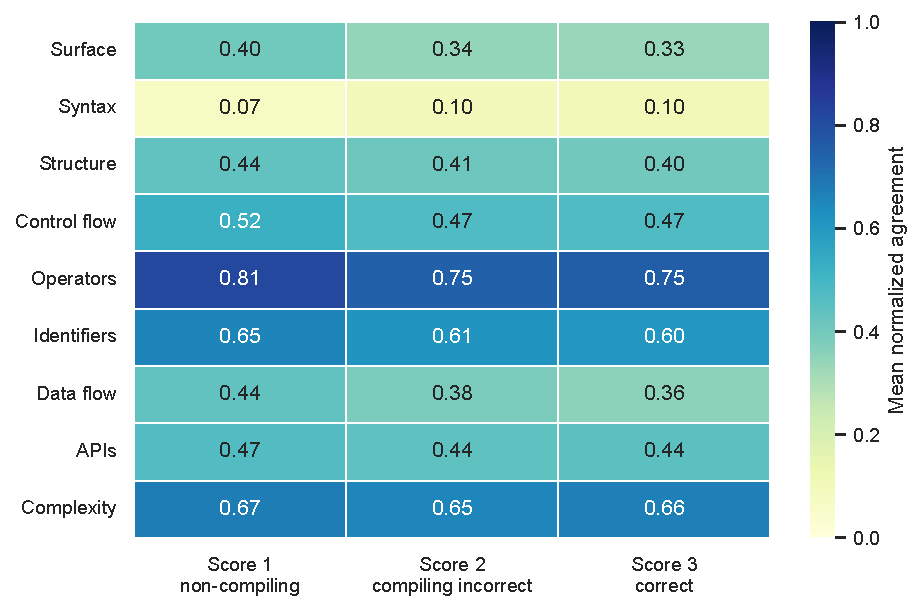
\includegraphics[width=.58\textwidth]{quality_progression_heatmap.pdf}
\caption{Domain-macro mean family agreement by execution grade. Most families do not increase with behavioral quality. Syntax is the exception in aggregate, although its zero values outside Python also reflect parser availability.}
\label{fig:progression}
\end{figure*}

\subsection{Traceability and Illustrative Cases}
\label{sec:explanation-failures}
Named probes make model use inspectable, but inspectability is not the same as a validated causal explanation. Correlation can change coefficient signs, and a lightweight extractor can misrepresent a source-language construct. We therefore use attribution to report which measured properties moved confidence, not why a program is behaviorally correct.

\begin{figure*}[t]
\centering
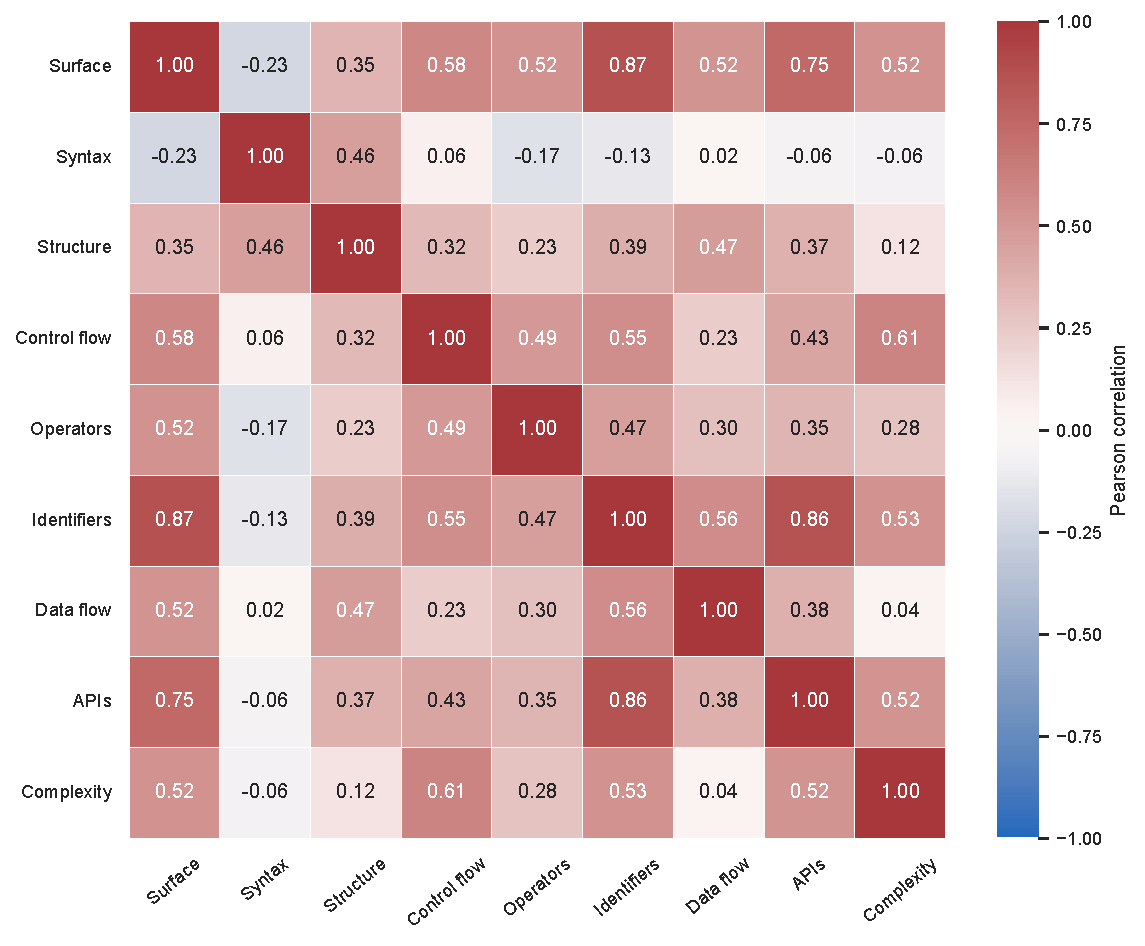
\includegraphics[width=.46\textwidth]{family_correlation.pdf}\hspace{.025\textwidth}
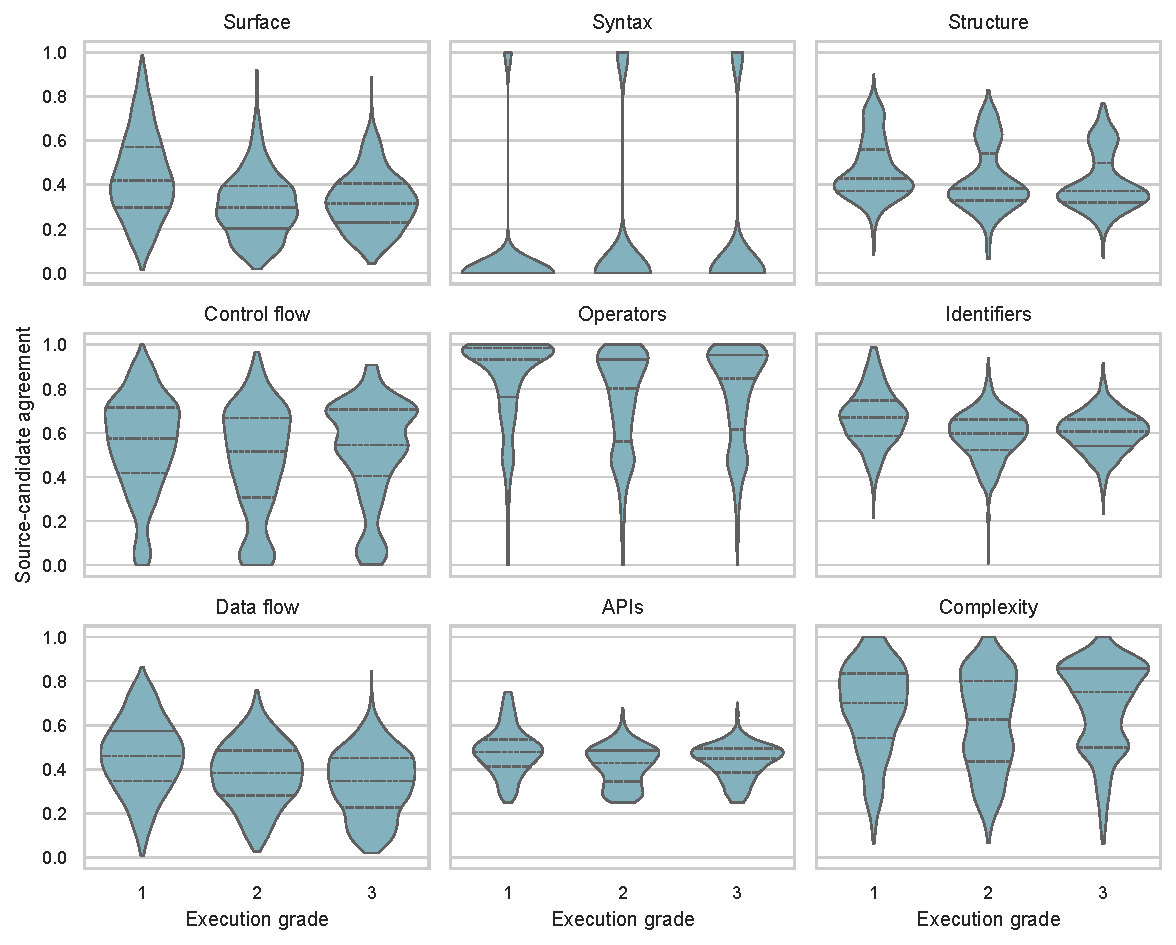
\includegraphics[width=.46\textwidth]{family_grade_distributions.pdf}
\caption{Why no observation family is decisive. The left panel measures held-out family-mean correlation, which identifies potential replacement. The right panel shows family-agreement distributions by execution grade. Broad overlap demonstrates that no family is a standalone correctness scale.}
\label{fig:evidence-dependence}
\end{figure*}

Figure~\ref{fig:evidence-dependence} explains why contribution and ablation rankings differ. Surface and identifiers correlate at $r=0.87$, identifiers and APIs at $r=0.86$, and control and complexity at $r=0.61$, so one family can partly replace another. In contrast, data flow and complexity correlate at only $r=0.04$, while syntax and data flow correlate at $r=0.02$, allowing modest features to add distinct warnings. The observed pattern reflects a combination of shared and complementary information across probe families. Some families capture overlapping aspects of source--candidate compatibility, whereas others contribute information that is only partially redundant. As a result, removing any single family reduces performance only modestly, with the ROC-AUC remaining at or above 0.781 in every case. This behaviour indicates that the representation degrades gracefully when one source of evidence is removed. At the same time, it should not be interpreted as evidence that the probe families are statistically independent or that any individual family is unnecessary.

The violin plots provide complementary insight into this behaviour. Every correctness grade exhibits a broad distribution of static semantic agreement rather than a narrowly defined score range. Consequently, no individual probe family serves as a reliable surrogate for overall translation quality. Instead, meaningful assessment emerges from combining evidence across multiple families, each contributing a different perspective on semantic compatibility.

The held-out artifact also preserves 25 high-confidence incorrect and 25 low-confidence correct threshold extremes for inspection. We do not treat this convenience sample as a coded qualitative study. Figure~\ref{fig:ambiguity-cases} instead presents two deliberately selected held-out programs with nearly equal scores but opposite outcomes. Their contrast shows that observation profiles can expose support and warnings while still failing to determine correctness.

\textbf{Answer to RQ3.} The 45 probes are the nonduplicate pairwise output of a declared, outcome-blind construct process. Primary AUC remains between 0.787 and 0.790 under correlation pruning, parser-channel removal, and duplicate restoration. SHAP, MI, and ablation show different forms of conditional use, marginal association, and replacement, while every single-family ablation retains at least 0.781 AUC. EviCode-XGB reaches 0.854, compared with 0.869 for the strongest frozen encoder under the common protocol. The explicit representation is therefore close in ranking while offering named program-property attribution through EviCode-LR. RQ4 next tests whether the learned relationships transport across domains.

\FloatBarrier
\section{RQ4: Which Relationships Transport?}
\label{sec:rq4}
RQ4 uses two complementary generalization protocols. The pairwise matrices train on one domain and evaluate another while preserving the global problem-disjoint split. They test single-domain transport to unseen tasks. The LOGO studies instead provide external model and domain validation: leave-one-generator-out asks whether relationships learned from two generators remain useful for a previously unseen generator, and leave-one-language-out asks whether the same observation basis remains useful after excluding an entire source language from training. LOGO can encounter the same programming tasks through other domains, so it measures domain exclusion rather than simultaneous task and domain novelty. Neither protocol isolates language normalization causally because the full representation also contains surface and lower-level probes.

Figure~\ref{fig:generator-transfer-matrix} first shows problem-disjoint generator transport. DeepSeek-Coder$\rightarrow$StarCoder is near random at 0.548, while QwenCoder$\rightarrow$StarCoder reaches 0.696. The same target generator can therefore be easier or harder depending on the training generator. This asymmetry supports a narrow conclusion: generator domains have different feature--label relationships. It does not reveal the models' internal reasoning process.

\begin{table}[t]
\centering
\caption{Leave-one-generator-out external model generalization. Each model is retrained without the evaluated generator, testing whether semantic relationships learned from two LLM families remain useful for a previously unseen generator.}
\label{tab:generator}
\begin{tabular}{@{}lrr@{}}
\toprule
Held-out generator & $n$ & LOGO AUC \\
\midrule
DeepSeek-Coder & 11,404 & 0.686 \\
QwenCoder & 8,935 & 0.749 \\
StarCoder & 10,640 & 0.655 \\
\bottomrule
\end{tabular}
\end{table}

Table~\ref{tab:generator} complements the pairwise matrix with an external generator-generalization study. Excluding one generator still yields AUC 0.655--0.749, so associations learned from two LLM families retain useful ordering on a previously unseen generator. Because LOGO and pooled subgroup evaluation use different task populations, we do not interpret their difference as the causal effect of exclusion. The defensible result is partial model-family generalization with substantial generator dependence.

\begin{figure}[t]
\centering
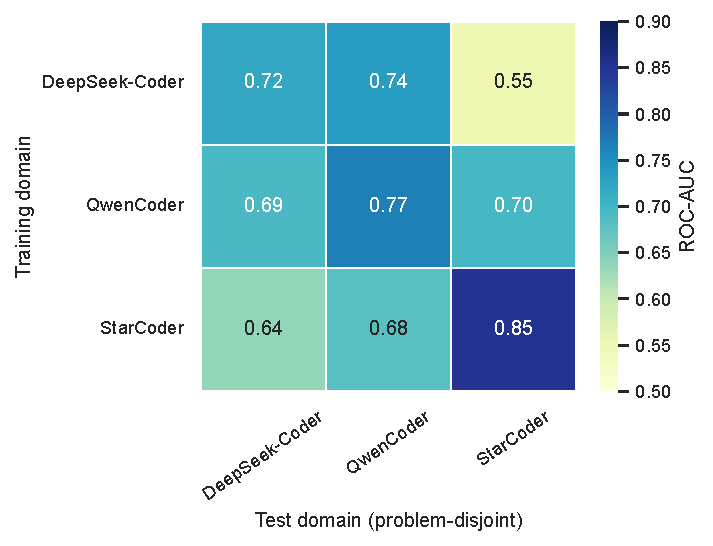
\includegraphics[width=\linewidth]{generator_transfer_matrix.pdf}
\caption{Problem-disjoint pairwise generator transport. Each cell is ROC-AUC after training on the row generator's training problems and evaluating the column generator's unseen test problems. Off-diagonal asymmetry shows that feature--label relationships differ across generators.}
\label{fig:generator-transfer-matrix}
\end{figure}

\begin{figure*}[t]
\centering
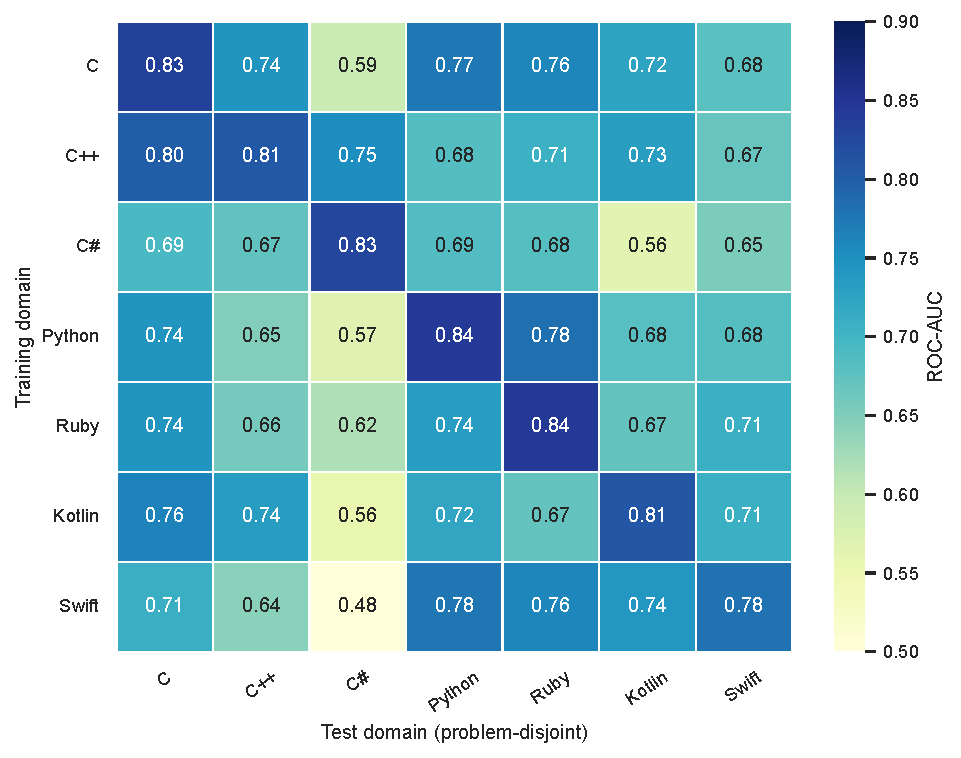
\includegraphics[width=.50\textwidth]{language_transfer_matrix.pdf}
\caption{Problem-disjoint pairwise source-language transport. Each cell trains on one source language and evaluates another on unseen problems, with Java fixed as the target. Values above 0.5 indicate useful ordering, while asymmetric cells expose language-specific limits.}
\label{fig:language-transfer-matrix}
\end{figure*}

Figure~\ref{fig:language-transfer-matrix} asks whether the extracted relationships survive a change in source-language syntax while Java remains the target. Useful ordering persists across many pairs. C-trained EviCode-LR reaches 0.775 on Python, and Python-trained EviCode-LR reaches 0.782 on Ruby. The exceptions define the boundary. C-trained evidence reaches only 0.595 on C\#, and Swift-trained evidence falls below chance on C\# at 0.484. The matrix is consistent with partial transport of shared relations, but cannot distinguish normalized semantics from stable Java-side, task, or generator regularities.

\begin{figure*}[t]
\centering
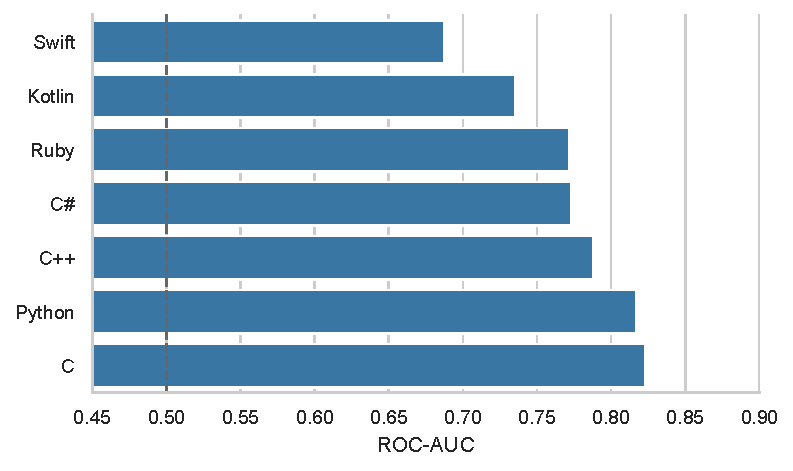
\includegraphics[width=.43\textwidth]{language_wise_auc.pdf}\hspace{.035\textwidth}
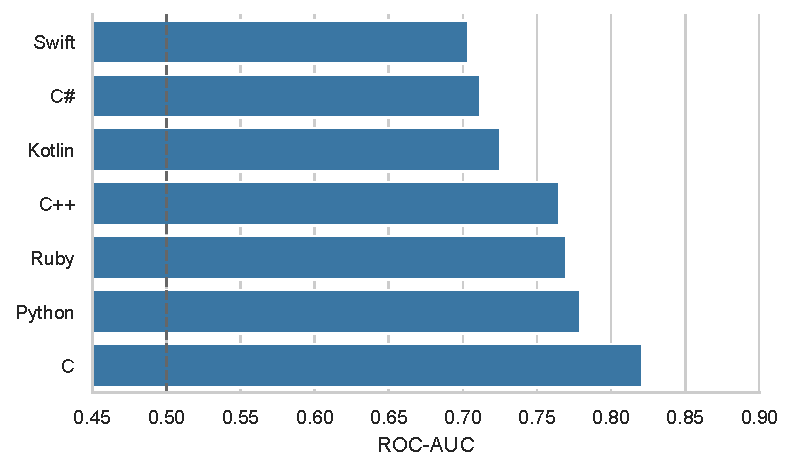
\includegraphics[width=.43\textwidth]{logo_language_auc.pdf}
\caption{Source-language external domain validation for EviCode-LR. The left panel reports pooled-model AUC within each held-out language subgroup (0.687--0.823). The right panel reports leave-one-language-out validation (0.704--0.821), where an entire source language is excluded during training.}
\label{fig:language-summary}
\end{figure*}

Figure~\ref{fig:language-summary} adds external source-domain validation. Pooled-model subgroup AUC on unseen problems ranges from 0.687 to 0.823. Leave-one-language-out AUC remains 0.704--0.821 when an entire source language is excluded from training, showing that the learned relationships are not wholly tied to having seen that language. Together with leave-one-generator-out AUC of 0.655--0.749, the results show useful generalization across held-out source domains and previously unseen generators. They do not establish target-language independence, because every candidate is Java.

\textbf{Answer to RQ4.} Explicit source--candidate relationships transport selectively across domains. Problem-disjoint matrices demonstrate useful cross-domain ordering on unseen tasks. LOGO analyses provide external validation by excluding an entire source language or code generator during training. Asymmetry and below-chance cells rule out universal invariance. The findings are consistent with partial transport of normalized computational relations within a fixed Java-target setting, not with complete language independence.

\subsection{Interpreting the Fixed-Target Design}
Languages differ in grammar, types, libraries, and idioms, yet reuse branches, iteration, returns, operators, definitions, uses, and calls. EviCode compares these extracted concepts after language-specific normalization. Fixing Java makes Figure~\ref{fig:language-transfer-matrix} easier to interpret because candidate parsing, target APIs, compilation, and wrapper conventions do not change between cells. The same control creates a boundary. Stable Java-side regularities may contribute to transport, LOGO can retain familiar tasks, and the results therefore support partial source-domain transport rather than language-independent semantics.

Extending coverage is asymmetric. Adding a source language while retaining Java requires a deterministic front end that maps its constructs to the declared obligations, followed by extractor-validity and calibration checks. Adding a target language also changes candidate parsing, APIs, types, exceptions, wrapper conventions, the compiler and runtime, and the behavioral oracle. It therefore requires re-extraction, refitting, and renewed evaluation of feature usefulness, transfer, thresholds, and calibration rather than reuse of the Java-trained coefficients. A multi-target design would improve external validity and separate source, target, and source--target interactions. It would also divide data across more domains and risk measuring unequal extractor maturity unless front ends and outcome coverage are comparable. Exceptions, aliasing, numeric behavior, APIs, and refactorings remain particularly difficult to normalize.

These constraints define the scope of the transport finding. Since score ordering can survive even when a probability mapping changes, RQ5 examines confidence directly.

\FloatBarrier
\section{RQ5: When Does Evidence Support Probability?}
\label{sec:rq5}
A useful ranking does not necessarily imply meaningful probabilities. An estimator may order candidates correctly while remaining overconfident or underconfident. RQ5 asks whether an EviCode-LR score can be read as a probability, and for which distribution. Figure~\ref{fig:generator-reliability} first tests whether one confidence value means the same thing across generators. Figure~\ref{fig:pooled-reliability} then examines pooled reliability and score support. Finally, domain statistics and the conditional-task ECE of 0.177 expose where probability meaning changes. No post-hoc calibration is applied.

\begin{figure*}[t]
\centering
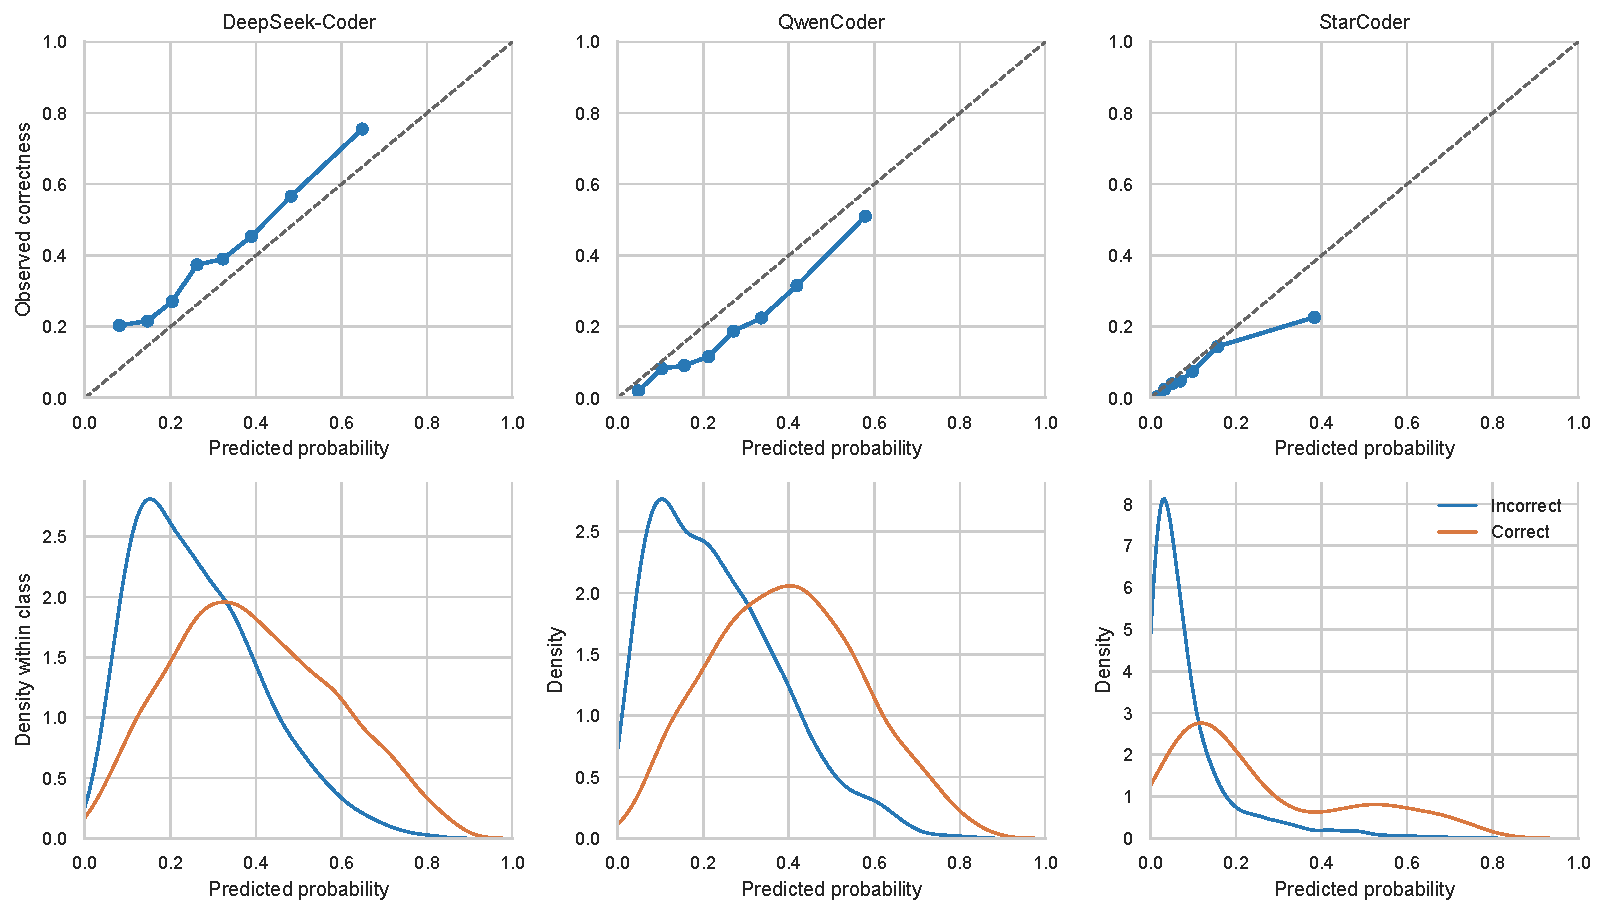
\includegraphics[width=.64\textwidth]{generator_reliability_and_scores.pdf}
\caption{Generator-specific reliability and score support from the pooled EviCode-LR model. Top panels use eight equal-frequency bins to compare confidence with observed correctness. Bottom panels normalize correct and incorrect densities separately. Different curves show that one score does not have generator-invariant meaning.}
\label{fig:generator-reliability}
\end{figure*}

Figure~\ref{fig:generator-reliability} shows that one numerical confidence occupies different reliability regimes and class-overlap patterns for each generator. A pooled threshold can therefore accept too many failures from one generator or reject too many correct programs from another. Calibration belongs to the model--deployment-distribution pair, not to the score alone.

\begin{figure*}[t]
\centering
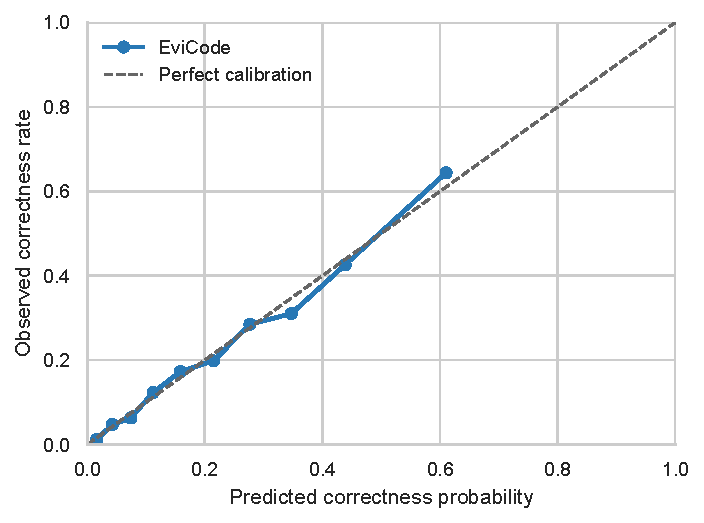
\includegraphics[width=.43\textwidth]{calibration.pdf}\hspace{.035\textwidth}
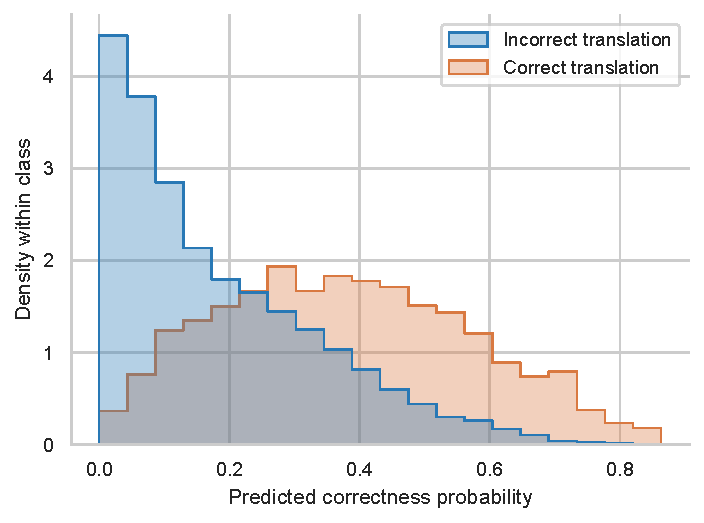
\includegraphics[width=.43\textwidth]{confidence_histogram.pdf}
\caption{Pooled EviCode-LR probability behavior on unseen problems. The left panel uses ten equal-frequency bins and shows reliability for the matched mixture. The right panel shows separately normalized score densities. Correct outputs shift higher, but broad overlap prevents any score range from becoming a certificate.}
\label{fig:pooled-reliability}
\end{figure*}

A perfectly calibrated estimator lies on the diagonal because predicted confidence then matches observed correctness. The left panel of Figure~\ref{fig:pooled-reliability} follows this relationship where the pooled test distribution contains sufficient observations. Its quantile bins differ from the ten equal-width bins used to compute ECE. The right panel confirms that correct candidates tend to receive higher confidence, but broad class overlap prevents a correctness certificate. Concentration in lower ranges also shows that pooled calibration is supported unevenly across the score domain.

\begin{table}[t]
\centering
\caption{Calibration for the pooled test set, all three generators, and Swift, the source language with the largest pooled-model ECE. Conf. is mean confidence, Prev. is prevalence, and ECE uses ten equal-width bins.}
\label{tab:calibration}
\begin{tabular}{@{}lrrrr@{}}
\toprule
Domain & $n$ & Conf. & Prev. & ECE \\
\midrule
Pooled & 9,482 & 0.229 & 0.228 & 0.011 \\
Swift & 354 & 0.240 & 0.407 & 0.183 \\
DeepSeek-Coder & 3,452 & 0.317 & 0.404 & 0.087 \\
QwenCoder & 2,819 & 0.266 & 0.193 & 0.074 \\
StarCoder & 3,211 & 0.103 & 0.070 & 0.032 \\
\bottomrule
\end{tabular}
\end{table}

Table~\ref{tab:calibration} explains why pooled ECE alone is insufficient. Pooled mean confidence nearly equals prevalence, a form of calibration in the large. At subgroup level, the same comparison indicates average underprediction for Swift and DeepSeek-Coder and average overprediction for QwenCoder and StarCoder. These differences are consistent with the grade distributions in Table~\ref{tab:data}. Calibration degradation does not mean that the ranking signal vanished. It means that the mapping from observed semantic evidence to probability of correctness changed under the conditioned population.

This distinction matters operationally. ROC-AUC depends primarily on relative ordering and can remain useful under distribution shift. Probability estimates and thresholds depend on prevalence and error composition. A model may therefore preserve triage value while requiring recalibration or locally selected thresholds before its probabilities can be interpreted reliably.

\textbf{Answer to RQ5.} Static semantic evidence can support probability-based triage only when the deployment distribution matches the validated calibration setting. On the pooled evaluation set, mean confidence (0.229) closely matches prevalence (0.228), ECE is 0.011, and populated quantile bins follow the ideal line. The conditioned and subgroup analyses show that this relationship changes with failure composition, language, and generator. Useful ranking may persist after probability meaning deteriorates, making local validation or recalibration necessary for deployment.

Taken together, the five RQs establish a consistent picture. The fixed semantic representation captures correctness-related information, but that information weakens among compiling candidates, is distributed across partially redundant probe families, transfers unevenly across languages and generators, and does not define a universal probability scale. The discussion therefore turns these findings into a bounded account of semantic observation.

\FloatBarrier
\section{Discussion}
\begin{figure*}[!t]
\centering
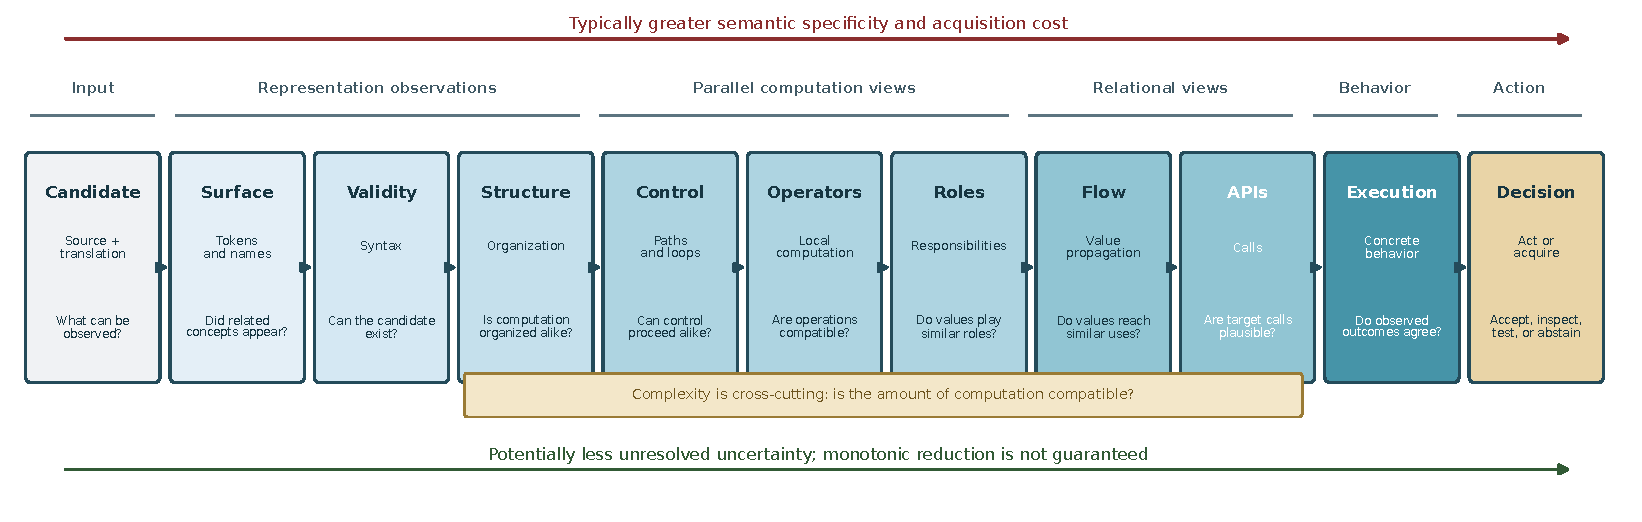
\includegraphics[width=\textwidth]{semantic_observability_continuum.pdf}
\caption{\textbf{Evidence acquisition timeline for semantic verification.} The source--candidate pair can be inspected through representation, computation, relation, and behavioral views before a decision is made. Later views are typically more semantically specific and costly, but the study does not measure a sequential policy or guarantee monotonic uncertainty reduction. Parallel boxes denote complementary rather than strictly ordered observations.}
\label{fig:continuum}
\end{figure*}

The predictive model itself is not the primary contribution. The contribution lies in the semantic representation constructed through the documented 53-to-49-to-45 process. The 45 nonduplicate pairwise observations form a transparent measurement instrument, not a complete description of program semantics or an optimized feature set. The matrix has full rank and no exact duplicate dimensions, yet substantial dependence remains among several probes. This fixed representation lets us ask which lightweight compatibility relations are associated with correctness, transferable across domains, attributable to interpretable observations, and still unobserved.

\subsection{The Semantic Information Ladder}
Figure~\ref{fig:continuum} summarizes the evidence accumulated across the five research questions. Section~\ref{sec:rq1} establishes static ranking ability (ROC-AUC $=0.790$). Section~\ref{sec:rq2} retains useful ordering among compiling candidates (ROC-AUC $=0.687$). Section~\ref{sec:rq3} shows distributed, partially replaceable support. Section~\ref{sec:rq4} examines language and generator transfer, and Section~\ref{sec:rq5} separates ranking from calibration. Together, these findings support verification as gradual accumulation of heterogeneous semantic observations rather than a single binary decision.

The ladder organizes semantic specificity, not predictive performance. API mismatch and call-name overlap have the largest EviCode-LR SHAP values in Section~\ref{sec:explanation-failures}, while control and APIs produce the largest point losses under family ablation. Syntax is nondecreasing across domains in Section~\ref{sec:quality-progression}, but parser availability makes most trajectories constant. The conditional AUC decline marks a change in evaluated failures, not an estimate of one rung's causal contribution. The ladder therefore describes \emph{what kind of program object is observed}. SHAP, MI, and ablation describe \emph{how this dataset and fitted instrument use its probes}. These are intentionally different orderings.

\subsection{What Execution-Grounded Supervision Teaches}
Constructed perturbations choose a defect mechanism in advance. Complete translation attempts can instead combine an invented API, omitted branch, confused accumulator, and plausible syntax. The distributed ablation and illustrative cases in Section~\ref{sec:rq3} are consistent with such interactions. No single-family removal lowers the point-estimate AUC below 0.781.

The semantic ladder should therefore be interpreted as an ordering of semantic specificity rather than predictive strength. Obligations contribute evidence from different perspectives, and confidence emerges from their combined agreement with successful behaviour. Disagreement provides complementary evidence against correctness. This distributed structure explains why no family dominates and why single-family removals cause only modest degradation.

The representation comparison in Section~\ref{sec:representation-ablation} reinforces this interpretation. Nonlinear interactions reduce the gap between EviCode and the strongest frozen pretrained encoder to approximately 0.016 ROC-AUC. EviCode-LR preserves attribution to named semantic observations, while EviCode-XGB shows the extra signal available from interactions. Attribution can identify measured contributors, such as operator disagreement or preserved control structure, but it does not prove perfect extraction or causal responsibility.

\begin{figure*}[!t]
\centering
\setlength{\fboxsep}{4pt}
\fcolorbox{black!35}{black!2}{%
\begin{minipage}[t][2.92in][t]{.46\textwidth}
\scriptsize
\textbf{Case A. Correct translation with incomplete support}\\[-1pt]
\textbf{Score 0.732, Grade 3}\quad
\textbf{Trace.} \texttt{deepseekcoder\_15421}, \texttt{p03563}\\[2pt]
\textbf{Python source}
\par\noindent\fcolorbox{black!12}{white}{\begin{minipage}{.96\linewidth}
\ttfamily\fontsize{6.3}{6.9}\selectfont
r = int(input())\\
g = int(input())\\
print(2 * g - r)
\end{minipage}}\par
\textbf{Java candidate}
\par\noindent\fcolorbox{black!12}{white}{\begin{minipage}{.96\linewidth}
\ttfamily\fontsize{6.3}{6.9}\selectfont
import java.util.*;\\
class Main \{\\
\hspace*{1em}public static void main(String[] args) \{\\
\hspace*{2em}Scanner scanner = new Scanner(System.in);\\
\hspace*{2em}int r = scanner.nextInt();\\
\hspace*{2em}int g = scanner.nextInt();\\
\hspace*{2em}System.out.println(2 * g - r);\\
\hspace*{1em}\}\\
\}
\end{minipage}}\par
\textbf{Observations.} Parses on both sides. Complexity agreement is 1.000 and operator agreement is 0.981, but identifier-role similarity is 0.167 because scanner boilerplate changes local context.\\[1pt]
\textbf{Reading.} The arithmetic is preserved, but wrapper code weakens identifier and structure agreement. The score is cautious about a correct program, not low because the translation is wrong.
\end{minipage}}
\hspace{.025\textwidth}
\fcolorbox{black!35}{black!2}{%
\begin{minipage}[t][2.92in][t]{.46\textwidth}
\scriptsize
\textbf{Case B. Plausible structure hides a defect}\\[-1pt]
\textbf{Score 0.742, Grade 2}\quad
\textbf{Trace.} \texttt{starcoder\_7336}, \texttt{p03067}\\[2pt]
\textbf{Python source}
\par\noindent\fcolorbox{black!12}{white}{\begin{minipage}{.96\linewidth}
\ttfamily\fontsize{6.3}{6.9}\selectfont
A, B, C = map(int, input().split())\\
if A < C < B or B < C < A:\\
\hspace*{1em}print("Yes")\\
else:\\
\hspace*{1em}print("No")
\end{minipage}}\par
\textbf{Java candidate}
\par\noindent\fcolorbox{black!12}{white}{\begin{minipage}{.96\linewidth}
\ttfamily\fontsize{6.3}{6.9}\selectfont
import java.util.*;\\
class Main \{\\
\hspace*{1em}public static void main(String[] args) \{\\
\hspace*{2em}Scanner sc = new Scanner(System.in);\\
\hspace*{2em}int a = sc.nextInt(), b = sc.nextInt();\\
\hspace*{2em}int c = sc.nextInt();\\
\hspace*{2em}if (a < c \&\& c < b \&\& b < a)\\
\hspace*{3em}System.out.println("Yes");\\
\hspace*{2em}else\\
\hspace*{3em}System.out.println("No");\\
\hspace*{1em}\}\\
\}
\end{minipage}}\par
\textbf{Observations.} Parses on both sides. Complexity and control agreement are 1.000, while identifier-role similarity is 0.067, expression density is 0.286, and operator agreement is 0.788.\\[1pt]
\textbf{Reading.} The candidate looks like a range check, but merges two valid orderings into an impossible conjunction. Static observations notice tension, yet do not execute the path condition, so the defect can still receive a similar score.
\end{minipage}}
\caption{\textbf{Held-out ambiguity cases with complete snippets.} Similar EviCode scores can arise from opposite outcomes because the score summarizes observed support and warning signals, not behavioral equivalence. The examples illustrate how named observations aid explanation while leaving residual uncertainty.}
\label{fig:ambiguity-cases}
\end{figure*}

\subsection{From Similarity to Semantic Evidence}
The three surface-level controls quantify token overlap, edit similarity, and program length without assuming semantic equivalence. Section~\ref{sec:rq1} shows that removing surface-level and validity-related observations reduces ROC-AUC only slightly, from 0.790 to 0.784, so most predictive signal comes from deeper semantic evidence. Still, normalized observations are informative summaries, not proofs. Section~\ref{sec:quality-progression} shows that only 21.7\% of probe-family/domain trajectories increase monotonically with correctness grade. Data flow does so in 4.8\%, and surface, structure, roles, APIs, and operators in 9.5\%. Correct refactoring can reduce similarity, while an incorrect boundary condition can preserve it almost completely. Correctness is not the endpoint of a similarity continuum.

\subsection{The Boundary of the Present Static Instrument}
Static observations such as branch counts, operators, calls, and definitions characterize structure but do not capture execution behaviour. Identical static profiles may still diverge because of one input-dependent branch, alias, overflow, exception path, or state update. No classifier using only the current vector can distinguish pairs that are identical in observation space. Compiling candidates therefore retain useful prioritization (ROC-AUC $=0.687$, precision $=0.778$), while ECE rises to 0.177. EviCode-XGB shows that richer fitting can exploit existing interactions, and stronger static or formal reasoning could refine the observation space. Behavioural evidence remains the strongest confirmation because it reveals concrete outcomes absent from these probes.

\subsection{Understanding Generator Shift}
Generators differ in literal preservation, control construction, library use, helper methods, and naming. These differences alter failure mixtures and change the mapping from semantic evidence to correctness. Because ranking depends mainly on relative compatibility, generator-specific LOGO evaluation still achieves ROC-AUC values between 0.655 and 0.749. Probability estimates also reflect prevalence and error composition, producing underconfidence for DeepSeekCoder and overconfidence for QwenCoder and StarCoder. Deployments should monitor generator drift and recalibrate on fresh execution-labelled samples when feasible.

\section{Implications for Reference-Free Verification}
The study suggests a staged architecture rather than a universal static gate. Preserve named observations so users can inspect which obligations support or contradict a candidate, use confidence to prioritize scarce review or testing resources, validate thresholds for the deployment language and generator, and acquire behavioral or formal evidence when unresolved risk justifies its cost. The present study motivates this policy but does not optimize sequential acquisition.

This architecture changes the verifier's question. It should not ask only, ``Is this program correct?'' It should instead ask which obligations have been observed, which remain uncertain, whether the confidence is valid for this distribution, and which next observation would most reduce consequential uncertainty. Such systems would treat abstention and evidence acquisition as successful outcomes rather than force static plausibility into a certificate.

For research, complete generator outputs and controlled fault probes remain complementary. This study analyzes the former and does not experimentally compare both settings.

\section{Threats to Validity}
\textbf{Construct validity.} Score 3 denotes success under the dataset oracle, not proof of equivalence. The 45-probe set is a bounded operationalization, not a complete or uniquely optimal basis for program semantics. The 53-to-45 process removes unilateral shortcuts and exact duplicates without consulting outcomes. The retained matrix has full rank, but 12 highly correlated pairs show that independence is neither achieved nor required. Parser-backed source profiles are available only for Python. Pooled AUC remains 0.788 after removing parser-dependent and fallback channels, but this does not establish equal extraction validity across languages. We do not independently annotate every extracted role, flow, or API relation. The instrument also omits full types, aliasing, heap state, exceptions, and path sensitivity. ``Evidence'' means empirical support under this instrument, never proof.

\textbf{Internal validity.} Generator and problem distributions may correlate with feature patterns despite metadata exclusion. The primary split is problem-disjoint but uses one random seed. Clustered bootstrap intervals resample test problems without refitting, so they quantify test-sample uncertainty conditional on one fitted model. LOGO holdouts can contain tasks represented in another domain and must not be read as simultaneous unseen-domain and unseen-problem tests. The 35-combination representation matrix makes no multiplicity-adjusted claim about its selected maximum.

\textbf{External validity.} Seven source languages vary, but Java is the only target. This control improves source-language comparisons while allowing Java-side regularities to contribute signal. Source-language holdout therefore tests unseen source syntax within one target ecosystem. It does not validate reverse direction, target-language transfer, or identical behavior for Java$\rightarrow$Python, Python$\rightarrow$C++, or C++$\rightarrow$Rust. Target APIs, type systems, runtimes, wrappers, oracles, and extractor maturity can change both observations and their usefulness. Measurements, thresholds, and calibration require validation for every new target.

\textbf{Conclusion validity.} AP and threshold metrics depend on prevalence, and pooled ECE can hide subgroup error. Reliability plots use quantile bins while ECE uses equal-width bins, and neither includes uncertainty intervals. The frozen encoders are truncated, mean-pooled, and not fine-tuned, so the comparison is controlled rather than state of the art. Bootstrap intervals do not account for oracle uncertainty, learner instability, or model-selection multiplicity.

\section{Reproducibility}
The repository contains the configurations, extraction and selection manifests, splits, fitted EviCode-LR model, predictions, bootstrap summaries, baselines, representation--learner outputs, frozen embeddings, ablations, progression results, illustrative cases, and figure scripts. Seed 42 is fixed, and labels, execution outcomes, compiler outcomes, generators, and problem identifiers are excluded from the feature matrix.

\section{Conclusion}
The findings presented in this work suggest that correctness cannot be characterized by a single template or signature of valid code. Instead, it emerges from the collective compatibility of multiple semantic properties, including program validity, structural organization, control flow, operator usage, value responsibilities, information propagation, API interactions, and computational complexity. The comparison between learning algorithms further shows that nonlinear models exploit interactions among these observations more effectively, whereas EviCode-LR retains the advantage of directly attributing predictions to interpretable program properties. Although the learned relationships generalize across programming languages and code generators to a meaningful extent, calibration and decision thresholds remain considerably more sensitive to changes in the underlying data distribution.

The study also clarifies the limits of what can be inferred from the current static representation. The proposed probes provide useful evidence for estimating translation plausibility, identifying semantic inconsistencies, prioritizing candidates for further inspection, and explaining which measured properties contributed to a prediction. However, they cannot directly observe the runtime behaviour that distinguishes many compiling yet incorrect translations from genuinely correct ones. While richer static analyses or formal reasoning could further refine the representation, behavioural evidence obtained through execution remains the strongest form of validation because it reveals program outcomes that are fundamentally inaccessible to the current observation space.

More broadly, these results motivate a different perspective on reference-free verification. Rather than asking only whether a generated program is correct, it is more informative to ask what evidence has been observed, how much uncertainty remains, whether the resulting confidence is valid for the current deployment setting, and what additional evidence would most effectively reduce that uncertainty. Within this perspective, language-normalized semantic probes provide an interpretable basis for prioritizing and diagnosing generated code when stronger evidence is unavailable, without claiming to establish correctness. Overall, the results indicate that explicit semantic observations recover a substantial proportion of the correctness-related information available under a strict static inference boundary while also making clear where static evidence alone reaches its inherent limits.

\begingroup
\let\oldthebibliography\thebibliography
\let\endoldthebibliography\endthebibliography
\renewenvironment{thebibliography}[1]{\oldthebibliography{#1}\normalsize}{\endoldthebibliography}
\setlength{\itemsep}{0pt}
\def\IEEEbibitemsep{0pt plus 0.2pt}
\bibliographystyle{IEEEtran}
\bibliography{references_v2}
\endgroup
\end{document}
